\chapter{Coxeter Groups and Tits Systems}

\section{COXETER GROUPS}

In this section, W denotes a group written multiplicatively, with identity element 1, and S denotes a set of generators of W such that \(S = S^{-1}\) and \(1 \notin S\) . Every element of W is the product of a finite sequence of elements of S. From no. 3 onwards we assume that every element of S is of order 2.

\subsection{LENGTH AND REDUCED DECOMPOSITIONS}

DEFINITION 1. Let \(w \in W\) . The length of \(w\) (with respect to \(S\) ), denoted by \(l_{S}(w)\) or simply by \(l(w)\) , is the smallest integer \(q \geqslant 0\) such that \(w\) is the product of a sequence of \(q\) elements of \(S\) . A reduced decomposition of \(w\) (with respect to \(S\) ) is any sequence \(s = (s_1, \ldots, s_q)\) of elements of \(S\) such that \(w = s_1 \ldots s_q\) and \(q = l(w)\) .

Thus 1 is the unique element of length 0 and \(S\) consists of the elements of length 1.

PROPOSITION 1. Let w and w' be in W. We have the formulas:

\[
l (w w ^ {\prime}) \leqslant l (w) + l (w ^ {\prime}),\tag{1}
\]

\[
l (w ^ {- 1}) = l (w),\tag{2}
\]

\[
\left| l (w) - l \left(w ^ {\prime}\right) \right| \leqslant l \left(w w ^ {\prime - 1}\right).\tag{3}
\]

Let \((s_{1},\ldots,s_{p})\) and \((s_{1}^{\prime},\ldots,s_{q}^{\prime})\) be reduced decompositions of w and \(w^{\prime}\) respectively. Thus \(l(w)=p\) and \(l(w^{\prime})=q\) . Since \(ww^{\prime}=s_{1}\ldots s_{p}s_{1}^{\prime}\ldots s_{q}^{\prime}\) , we have \(l(ww^{\prime})\leqslant p+q\) , proving (1). Since \(S=S^{-1}\) and \(w^{-1}=s_{p}^{-1}\ldots s_{1}^{-1}\) , we have \(l(w^{-1})\leqslant p=l(w)\) . Replacing w by \(w^{-1}\) gives the opposite inequality \(l(w)\leqslant l(w^{-1})\) , proving (2). Replacing w by \(ww^{\prime-1}\) in (1) and (2) gives the relations

\[
l (w) - l \left(w ^ {\prime}\right) \leqslant l \left(w w ^ {\prime - 1}\right),\tag{4}
\]

\[
l \left(w w ^ {\prime - 1}\right) = l \left(w ^ {\prime} w ^ {- 1}\right).\tag{5}
\]

Exchanging \(w\) and \(w'\) in (4) gives \(l(w') - l(w) \leqslant l(ww'^{-1})\) by (5), proving (3).

COROLLARY. Let \(\mathbf{s} = (s_{1}, \ldots, s_{p})\) and \(\mathbf{s}' = (s_{1}', \ldots, s_{q}')\) be two sequences of elements of S such that \(w = s_{1} \ldots s_{p}\) and \(w' = s_{1}' \ldots s_{q}'\) . If the sequence \((s_{1}, \ldots, s_{p}, s_{1}', \ldots, s_{q}')\) is a reduced decomposition of \(ww'\) , then s is a reduced decomposition of w and \(s'\) is one of \(w'\) .

By hypothesis, \(l(w) \leqslant p\) , \(l(w') \leqslant q\) and \(l(ww') = p + q\) . By (1), we must have \(l(w) = p\) and \(l(w') = q\) , hence the corollary.

Remark In view of formulas (1) and (2), the formula \(d(w, w') = l(ww'^{-1})\) defines a distance on W, invariant under right translations.

\subsection{DIHEDRAL GROUPS}

DEFINITION 2. A dihedral group is a group generated by two distinct elements of order two.

Example. Let M be the multiplicative group \(\{1,-1\}\) , and let m be an integer \(\geqslant2\) (resp. \(m=\infty\) ). Then M acts on the group Z/mZ (resp. on Z) by \((-1).x=-x\) , and the corresponding semi-direct product of M by Z/mZ (resp. of M by Z) is denoted by \(D_{m}\) . The elements of \(D_{m}\) are thus the pairs \((\varepsilon,x)\) with \(\varepsilon=\pm1\) and \(x\in Z/mZ\) (resp. \(x\in Z\) ); the group law on \(D_{m}\) is given by the formula

\[
(\varepsilon , x). (\varepsilon^ {\prime}, x ^ {\prime}) = (\varepsilon \varepsilon^ {\prime}, \varepsilon^ {\prime} x + x ^ {\prime}).\tag{6}
\]

We denote by \(\iota\) the class of 1 modulo \(m\) (resp. \(\iota = 1\) ) and set

\[
\rho = (- 1, 0), \quad \rho^ {\prime} = (- 1, \iota), \quad \pi = (1, \iota).\tag{7}
\]

Then \(\rho^2 = \rho'^2 = 1\) and \(\pi = \rho \rho'\) . The formulas

\[
\pi^ {n} = (1, n \iota), \quad \rho \pi^ {n} = (- 1, n \iota)\tag{8}
\]

show that \(D_{m}\) is a dihedral group generated by \(\{\rho,\rho'\}\) .

PROPOSITION 2. Assume that \(S\) consists of two distinct elements \(s\) and \(s'\) of order 2.

\begin{enumerate}
\def\labelenumi{(\roman{enumi})}
\item
  The subgroup P of W generated by \(p = ss'\) is normal, and W is the semi-direct product of the subgroup \(T = \{1, s\}\) and P. Moreover, \((W : P) = 2\) .
\item
  Let \(m\) be the order (finite or infinite) of \(p\) . Then \(m \geqslant 2\) and \(W\) is of order \(2m\) . There is a unique isomorphism \(\varphi\) from \(D_m\) to \(W\) such that \(\varphi(\rho) = s\) and \(\varphi(\rho') = s'\) .
\item
  We have \(sps^{-1} = sss's = s's = p^{-1}\) , and hence
\end{enumerate}

\[
s p ^ {n} s ^ {- 1} = p ^ {- n}\tag{9}
\]

for every integer \(n\) . Since \(W\) is generated by \(\{s, s'\}\) , and hence by \(\{s, p\}\) , the subgroup \(P\) is normal. It follows that \(TP\) is a subgroup of \(W\) , and since \(TP\) contains \(s\) and \(s' = sp\) , we have \(W = TP = P \cup sP\) . To prove (i), it is therefore enough to show that \(W \neq P\) . If \(W = P\) , the group \(W\) would be commutative, so \(p^2 = s^2 s'^2 = 1\) . But then the only elements of \(W = P\) would be 1 and \(p\) , contradicting the hypothesis that \(W\) contains at least three elements, namely 1, \(s\) and \(s'\) .

\begin{enumerate}
\def\labelenumi{(\roman{enumi})}
\setcounter{enumi}{1}
\tightlist
\item
  Since \(s \neq s'\) , we have \(p \neq 1\) and so \(m \geqslant 2\) . Since P is of order m and (W : P) = 2, the order of W is 2m. If m is finite (resp. infinite), there exists an isomorphism \(\varphi'\) from Z/mZ (resp. Z) to P taking \(\pi\) to p.~Moreover, there exists an isomorphism \(\varphi''\) from M = \{1, -1\} to T taking -1 to s. The group W is the semi-direct product of T and P. In view of the formulas (9) and \(\rho\pi^{n}\rho^{-1} = \pi^{-n}\) , \(\varphi'\) and \(\varphi''\) induce an isomorphism \(\varphi\) from D\_\{m\} to W such that \(\varphi(\rho) = s\) and \(\varphi(\pi) = p\) , and hence \(\varphi(\rho') = s'\) . The uniqueness of \(\varphi\) follows from the fact that D\_\{m\} is generated by \(\{\rho, \rho'\}\) .
\end{enumerate}

Remark. Consider a dihedral group W of order 2m generated by two distinct elements s and \(s'\) of order 2. Denote by \(s_{q}\) (resp. \(s'_{q}\) ) the sequence of length q whose odd (resp. even) numbered terms are equal to s and whose even (resp. odd) numbered terms are equal to \(s'\) , and let \(w_{q}\) (resp. \(w'_{q}\) ) be the product of the sequence \(s_{q}\) (resp. \(s'_{q}\) ). We have

\[
\begin{array}{r l} w _ {2 k} = (s s ^ {\prime}) ^ {k}, & w _ {2 k + 1} = (s s ^ {\prime}) ^ {k} s, \\ w _ {2 k} ^ {\prime} = (s ^ {\prime} s) ^ {k} = (s s ^ {\prime}) ^ {- k}, & w _ {2 k + 1} ^ {\prime} = (s ^ {\prime} s) ^ {k} s ^ {\prime} = (s s ^ {\prime}) ^ {- k - 1} s. \end{array}
\]

If \(\mathbf{s} = (s_1, \ldots, s_q)\) is a reduced decomposition (with respect to \(\{s, s'\}\) ) of an element \(w\) of W, then clearly \(s_i \neq s_{i+1}\) for \(1 \leqslant i \leqslant q-1\) . Hence, \(\mathbf{s} = \mathbf{s}_q\) or \(\mathbf{s} = \mathbf{s}_q'\) .

If \(m = \infty\) , the elements \((ss')^n\) and \((ss')^ns\) for \(n \in \mathbf{Z}\) are distinct. Hence, the elements \(w_q\) ( \(q \geqslant 0\) ) and \(w_q'\) ( \(q > 0\) ) are distinct, and if \(\mathbf{s}\) is a reduced decomposition of \(w_q\) (resp. \(w_q'\) ) we necessarily have \(\mathbf{s} = \mathbf{s}_q\) (resp. \(\mathbf{s} = \mathbf{s}_q'\) ). It follows from this that \(l(w_q) = l(w_q') = q\) and that the set of reduced decompositions of the elements of \(\mathbf{W}\) consists of the \(\mathbf{s}_q\) and the \(\mathbf{s}_q'\) . Moreover, every element of \(\mathbf{W}\) has a unique reduced decomposition.

Suppose now that \(m\) is finite. If \(q \geqslant 2m\) , we have \(w_{q} = w_{q - 2m}\) and \(w_{q}' = w_{q - 2m}'\) ; if \(m \leqslant q \leqslant 2m\) , we have \(w_{q} = w_{2m - q}'\) , \(w_{q}' = w_{2m - q}\) . Hence, neither \(\mathbf{s}_q\) nor \(\mathbf{s}_q'\) are reduced decompositions if \(q > m\) . It follows that each of the \(2m\) elements of \(W\) is one of the \(2m\) elements \(w_0 = w_0'\) , \(w_q\) and \(w_q'\) for \(1 \leqslant q \leqslant m - 1\) , and \(w_m = w_m'\) . These \(2m\) elements are thus distinct and it follows as above that \(l(w_q) = l(w_q') = q\) for \(q \leqslant m\) and that the set of reduced decompositions of elements of \(W\) consists of the \(s_q\) and the \(s_q'\) for \(0 \leqslant q \leqslant m\) . Every element of \(W\) except \(w_m\) has a unique reduced decomposition; \(w_m\) has two.

\subsection{FIRST PROPERTIES OF COXETER GROUPS}

Recall that from now on we assume that the elements of S are of order 2.

DEFINITION 3. (W,S) is said to be a Coxeter system if it satisfies the following condition:

\begin{enumerate}
\def\labelenumi{(\Alph{enumi})}
\setcounter{enumi}{2}
\tightlist
\item
  For \(s, s'\) in \(S\) , let \(m(s, s')\) be the order of \(ss'\) and let \(I\) be the set of pairs \((s, s')\) such that \(m(s, s')\) is finite. The generating set \(S\) and the relations \((ss')^{m(s, s')} = 1\) for \((s, s')\) in \(I\) form a presentation \(^{1}\) of the group \(W\) .
\end{enumerate}

When (W,S) is a Coxeter system, one also says, by abuse of language, that W is a Coxeter group.

Examples. 1) Let \(m\) be an integer \(\geqslant 2\) or \(\infty\) and let \(W\) be a group defined by a set of generators \(S = \{s, s'\}\) and the relations \(s^2 = s'^2 = 1\) when \(m = \infty\) , \(s^2 = s'^2 = (ss')^m = 1\) when \(m\) is finite. Consider on the other hand the dihedral group \(D_m\) (no. 2, Example) and the elements \(\rho\) and \(\rho'\) of \(D_m\) defined by (7). Since \(\rho^2 = \rho'^2 = 1\) and \((\rho \rho')^m = 1\) when \(m\) is finite, there exists a unique homomorphism \(f\) from \(W\) to \(D_m\) such that \(f(s) = \rho\) and \(f(s') = \rho'\) . Since \(\rho \rho'\) is of order \(m\) , it follows that \(ss'\) is itself of order \(m\) . Hence, \((W, S)\) is a Coxeter system, \(W\) is a dihedral group of order \(2m\) and \(f\) is an isomorphism (Prop. 2).

By transport of structure, it follows that every dihedral group is a Coxeter group.

\begin{enumerate}
\def\labelenumi{\arabic{enumi})}
\setcounter{enumi}{1}
\item
  Let \(\mathfrak{S}_n\) be the symmetric group of degree \(n\) , with \(n \geqslant 2\) . Let \(s_i\) be the transposition of \(i\) and \(i + 1\) for \(1 \leqslant i < n\) , and let \(S = \{s_1, \ldots, s_{n-1}\}\) . One can show (§2, no.4, Example and §1, Exerc. 4) that \((\mathfrak{S}_n, S)\) is a Coxeter system.
\item
  For the classification of finite Coxeter groups, cf.~Chap. 4, § 4.
\end{enumerate}

Remark. Suppose that \((W,S)\) is a Coxeter system. There exists a homomorphism \(\varepsilon\) from W to the group \(\{1,-1\}\) characterized by \(\varepsilon(s)=-1\) for all \(s\in S\) . We call \(\varepsilon(w)\) the signature of w; it is equal to \((-1)^{l(w)}\) . The formula \(\varepsilon(ww')=\varepsilon(w)\varepsilon(w')\) thus translates into \(l(ww')\equiv l(w)+l(w')\) mod. 2.

PROPOSITION 3. Assume that (W, S) is a Coxeter system. Then, two elements s and s' of S are conjugate \(^{2}\) in W if and only if the following condition is satisfied:

\begin{enumerate}
\def\labelenumi{(\Roman{enumi})}
\tightlist
\item
  There exists a finite sequence \((s_1, \ldots, s_q)\) of elements of \(S\) such that \(s_1 = s, s_q = s'\) and \(s_j s_{j+1}\) is of finite odd order for \(1 \leqslant j < q\) .
\end{enumerate}

Let \(s\) and \(s'\) in \(S\) be such that \(p = ss'\) is of finite order \(2n + 1\) . By (9), \(sp^{-n} = p^n s\) hence

\[
p ^ {n} s p ^ {- n} = p ^ {n} p ^ {n} s = p ^ {- 1} s = s ^ {\prime} s s = s ^ {\prime},\tag{10}
\]

and \(s'\) is conjugate to \(s\) .

For all s in S, let \(A_{s}\) be the set of \(s' \in S\) satisfying (I). With the hypotheses in (I), the elements \(s_{j}\) and \(s_{j+1}\) are conjugate for \(1 \leqslant j < q\) by the above, hence every element \(s'\) of \(A_{s}\) is conjugate to s.

Let \(f\) be the map from \(S\) to \(M = \{1, -1\}\) equal to 1 on \(A_s\) and to -1 on \(S - A_s\) . Let \(s'\) and \(s''\) in \(S\) be such that \(s's''\) is of finite order \(m\) . Then \(f(s')f(s'') = 1\) if \(s'\) and \(s''\) are both in \(A_s\) or both in \(S - A_s\) . In the other case, \(f(s')f(s'') = -1\) , but \(m\) is even. Thus \((f(s')f(s''))^m = 1\) in all cases. Since \((W, S)\) is a Coxeter system, there exists a homomorphism \(g\) from \(W\) to \(M\) inducing \(f\) on \(S\) . Let \(s'\) be a conjugate of \(s\) . Since \(s\) belongs to the kernel of \(g\) , so does \(s'\) , hence \(f(s') = g(s') = 1\) and finally \(s' \in A_s\) . Q.E.D.

\subsection{REDUCED DECOMPOSITIONS IN A COXETER GROUP}

Suppose that \((W,S)\) is a Coxeter system. Let T be the set of conjugates in W of elements of S. For any finite sequence \(\mathbf{s}=(s_{1},\ldots,s_{q})\) of elements of S, denote by \(\Phi(\mathbf{s})\) the sequence \((t_{1},\ldots,t_{q})\) of elements of T defined by

\[
t _ {j} = \left(s _ {1} \dots s _ {j - 1}\right) s _ {j} \left(s _ {1} \dots s _ {j - 1}\right) ^ {- 1} \quad \text { for } 1 \leqslant j \leqslant q.\tag{11}
\]

Then \(t_1 = s_1\) and \(s_1 \ldots s_q = t_q t_{q-1} \ldots t_1\) . For any element \(t \in \mathbf{T}\) , denote by \(n(\mathbf{s}, t)\) the number of integers \(j\) such that \(1 \leqslant j \leqslant q\) and \(t_j = t\) . Finally, put

\[
R = \{1, - 1 \} \times T.
\]

Lemma 1. (i) Let \(w \in \mathbf{W}\) and \(t \in \mathbf{T}\) . The number \((-1)^{n(\mathbf{s},t)}\) has the same value \(\eta(w,t)\) for all sequences \(\mathbf{s} = (s_1, \ldots, s_q)\) of elements of \(S\) such that \(w = s_1 \ldots s_q\) .

\begin{enumerate}
\def\labelenumi{(\roman{enumi})}
\setcounter{enumi}{1}
\tightlist
\item
  For \(w \in \mathbf{W}\) , let \(\mathrm{U}_w\) be the map from \(\mathbf{R}\) to itself defined by
\end{enumerate}

\[
\mathrm{U} _ {w} (\varepsilon , t) = (\varepsilon . \eta (w ^ {- 1}, t), w t w ^ {- 1}) \quad (\varepsilon = \pm 1, t \in \mathrm{T}).\tag{12}
\]

The map \(w \mapsto \mathrm{U}_w\) is a homomorphism from \(\mathbf{W}\) to the group of permutations of \(\mathbb{R}\) .

For \(s \in S\) , define a map \(U_s\) from \(R\) to itself by

\[
\mathrm{U} _ {s} (\varepsilon , t) = \left(\varepsilon . (- 1) ^ {\delta_ {s, t}}, s t s ^ {- 1}\right) \quad (\varepsilon = \pm 1, t \in \mathrm{T}),\tag{13}
\]

where \(\delta_{s,t}\) is the Kronecker symbol. It is immediate that \(U_{s}^{2} = Id_{R}\) , which shows that \(U_{s}\) is a permutation of R.

Let \(\mathbf{s} = (s_1, \ldots, s_q)\) be a sequence of elements of \(S\) . Put \(w = s_q \ldots s_1\) and \(U_{\mathbf{s}} = U_{s_q} \ldots U_{s_1}\) . We shall show, by induction on \(q\) , that

\[
\mathrm{U} _ {\mathbf {s}} (\varepsilon , t) = (\varepsilon . (- 1) ^ {n (\mathbf {s}, t)}, w t w ^ {- 1}).\tag{14}
\]

This is clear for \(q = 0,1\) . If \(q > 1\) , put \(\mathbf{s}' = (s_1,\dots ,s_{q - 1})\) and

\[
w ^ {\prime} = s _ {q - 1} \dots s _ {1}.
\]

Using the induction hypothesis, we obtain

\[
\begin{array}{r l} \mathrm{U} _ {\mathbf {s}} (\varepsilon , t) & = \mathrm{U} _ {s _ {q}} (\varepsilon . (- 1) ^ {n (\mathbf {s} ^ {\prime}, t)}, w ^ {\prime} t w ^ {\prime - 1}) \\ & = (\varepsilon . (- 1) ^ {n (\mathbf {s} ^ {\prime}, t) + \delta_ {s _ {q}, w ^ {\prime} t w ^ {\prime - 1}}}, w t w ^ {- 1}). \end{array}
\]

But \(\Phi(\mathbf{s}) = (\Phi(\mathbf{s}'), w'^{-1}s_q w')\) and \(n(\mathbf{s}, t) = n(\mathbf{s}', t) + \delta_{w'^{-1}s_q w', t}\) , proving formula (14).

Now let \(s, s' \in S\) be such that \(p = ss'\) has finite order \(m\) . Let \(\mathbf{s} = (s_1, \ldots, s_{2m})\) be the sequence of elements of \(S\) defined by \(s_j = s\) for \(j\) odd and \(s_j = s'\) for \(j\) even. Then \(s_{2m} \ldots s_1 = p^{-m} = 1\) and formula (11) implies that

\[
t _ {j} = p ^ {j - 1} s \quad \text { for } 1 \leqslant j \leqslant 2 m.\tag{15}
\]

Since \(p\) is of order \(m\) , the elements \(t_1, \ldots, t_m\) are distinct and \(t_{j+m} = t_j\) for \(1 \leqslant j \leqslant m\) . For all \(t \in \mathbf{T}\) , the integer \(n(\mathbf{s}, t)\) is thus equal to 0 or 2 and (14) shows that \(\mathrm{U_s} = \mathrm{Id_R}\) . In other words, \((\mathrm{U_sU_{s'}})^m = \mathrm{Id_R}\) . Thus, by the definition of Coxeter systems, there exists a homomorphism \(w \mapsto \mathrm{U}_w\) from \(W\) to the group of permutations of \(R\) such that \(U_s\) is given by the right-hand side of (13). Then \(U_w = U_s\) for every sequence \(s = (s_1, \ldots, s_q)\) such that \(w = s_q \ldots s_1\) and Lemma 1 follows immediately from (14).

Lemma 2. Let \(\mathbf{s} = (s_1, \ldots, s_q)\) , \(\Phi(\mathbf{s}) = (t_1, \ldots, t_q)\) and \(w = s_1 \ldots s_q\) . Let \(\mathrm{T}_w\) be the set of elements of \(\mathrm{T}\) such that \(\eta(w, t) = -1\) . Then \(\mathbf{s}\) is a reduced decomposition of \(w\) if and only if the \(t_i\) are distinct, and in that case \(\mathrm{T}_w = \{t_1, \ldots, t_q\}\) and \(\operatorname{Card}(\mathrm{T}_w) = l(w)\) .

Clearly \(T_{w} \subset \{t_{1}, \ldots, t_{q}\}\) . Taking s to be reduced, it follows that \(\operatorname{Card}(T_{w}) \leqslant l(w)\) . Moreover, if the \(t_{i}\) are distinct, then \(n(\mathbf{s}, t)\) is equal to 1 or 0 according to whether t does or does not belong to \(\{t_{1}, \ldots, t_{q}\}\) . It follows that \(T_{w} = \{t_{1}, \ldots, t_{q}\}\) and that \(q = \operatorname{Card}(T_{w}) \leqslant l(w)\) , which implies that s is reduced. Suppose finally that \(t_{i} = t_{j}\) with i \textless{} j. This gives \(s_{i} = us_{j}u^{-1}\) , with \(u = s_{i+1} \ldots s_{j-1}\) , hence

\[
w = s _ {1} \dots s _ {i - 1} s _ {i + 1} \dots s _ {j - 1} s _ {j + 1} \dots s _ {q}.
\]

This shows that s is not a reduced decomposition of w.

Lemma 3. Let \(w \in \mathbb{W}\) and \(s \in \mathbb{S}\) be such that \(l(sw) \leqslant l(w)\) . For any sequence \(\mathbf{s} = (s_1, \ldots, s_q)\) of elements of \(\mathbb{S}\) with \(w = s_1 \ldots s_q\) , there exists an integer \(j\) such that \(1 \leqslant j \leqslant q\) and

\[
s s _ {1} \dots s _ {j - 1} = s _ {1} \dots s _ {j - 1} s _ {j}.
\]

Let \(p\) be the length of \(w\) and \(w' = sw\) . By the Remark of no. 3, \(l(w') \equiv l(w) + 1 \mod 2\) . The hypothesis \(l(w') \leqslant l(w)\) and the relation

\[
| l (w) - l (w ^ {\prime}) | \leqslant l (w w ^ {\prime - 1}) = l (s) = 1
\]

thus leads to \(l(w') = p - 1\) . Choose a reduced decomposition

\[
\left(s _ {1} ^ {\prime}, \ldots , s _ {p - 1} ^ {\prime}\right)
\]

of \(w'\) and put \(\mathbf{s} = (s, s_1', \ldots, s_{p-1}')\) and \(\Phi(\mathbf{s}') = (t_1', \ldots, t_p')\) . It is clear that \(\mathbf{s}'\) is a reduced decomposition of \(w\) and that \(t_1' = s\) . The elements \(t_1', \ldots, t_p'\) being distinct by Lemma 2, we have \(n(\mathbf{s}', s) = 1\) . Since \(w\) is the product of the sequence \(\mathbf{s}\) , we have \(n(\mathbf{s}, s) \equiv n(\mathbf{s}', s) \mod 2\) by Lemma 1, hence \(n(\mathbf{s}, s) \neq 0\) . Consequently, \(s\) is equal to one of the elements \(t_j\) of the sequence \(\Phi(\mathbf{s})\) , hence the lemma.

Remark. The set \(T_{w}\) defined in Lemma 2 consists of the elements of the form \(w''sw''^{-1}\) corresponding to the triples \((w', w'', s) \in W \times W \times S\) such that \(w = w''sw'\) and \(l(w') + l(w'') + 1 = l(w)\) .

\subsection{THE EXCHANGE CONDITION}

The ``exchange condition'' is the following assertion about (W, S):

\begin{enumerate}
\def\labelenumi{(\Alph{enumi})}
\setcounter{enumi}{4}
\tightlist
\item
  Let \(w \in W\) and \(s \in S\) be such that \(l(sw) \leqslant l(w)\) . For any reduced decomposition \((s_1, \ldots, s_q)\) of \(w\) , there exists an integer \(j\) such that \(1 \leqslant j \leqslant q\) and
\end{enumerate}

\[
s s _ {1} \dots s _ {j - 1} = s _ {1} \dots s _ {j - 1} s _ {j}.\tag{16}
\]

We assume in this number that \((W,S)\) satisfies (E). By Lemma 3, this is so if \((W,S)\) is a Coxeter system. The results of this number thus apply to Coxeter systems.

PROPOSITION 4. Let \(s \in S\) , \(w \in W\) and \(s = (s_1, \ldots, s_q)\) be a reduced decomposition of \(w\) . Then one of the following must hold:

\begin{enumerate}
\def\labelenumi{\alph{enumi})}
\item
  \(l(sw) = l(w) + 1\) and \((s, s_1, \ldots, s_q)\) is a reduced decomposition of sw.
\item
  \(l(sw) = l(w) - 1\) and there exists an integer \(j\) such that \(1 \leqslant j \leqslant q\) , \((s_1, \ldots, s_{j-1}, s_{j+1}, \ldots, s_q)\) is a reduced decomposition of \(sw\) and \((s, s_1, \ldots, s_{j-1}, s_{j+1}, \ldots, s_q)\) is a reduced decomposition of \(w\) .
\end{enumerate}

Put \(w' = sw\) . By formula (3) of no. 1, we have

\[
\left| l (w) - l \left(w ^ {\prime}\right) \right| \leqslant l (s) = 1.
\]

We distinguish two cases:

\begin{enumerate}
\def\labelenumi{\alph{enumi})}
\tightlist
\item
  \(l(w') > l(w)\) . Then \(l(w') = q + 1\) and \(w' = ss_1 \ldots s_q\) , so
\end{enumerate}

\[
\left(s, s _ {1}, \ldots , s _ {q}\right)
\]

is a reduced decomposition of \(w'\) .

\begin{enumerate}
\def\labelenumi{\alph{enumi})}
\setcounter{enumi}{1}
\tightlist
\item
  \(l(w') \leqslant l(w)\) . By (E), there exists an integer \(j\) such that \(1 \leqslant j \leqslant q\) and (16) is satisfied. Then \(w = ss_1 \ldots s_{j-1}s_{j+1} \ldots s_q\) and hence
\end{enumerate}

\[
w ^ {\prime} = s _ {1} \dots s _ {j - 1} s _ {j + 1} \dots s _ {q}.
\]

Since \(q - 1 \leqslant l(w') \leqslant q\) , it follows that \(l(w') = q - 1\) and that \((s_1, \ldots, s_{j-1}, s_{j+1}, \ldots, s_q)\) is a reduced decomposition of \(w'\) .

Lemma 4. Let \(w \in W\) have length \(q \geqslant 1\) , let \(D\) be the set of reduced decompositions of \(w\) , and let \(F\) be a map from \(D\) to a set \(E\) . Assume that \(F(s) = F(s')\) if the elements \(s = (s_1, \ldots, s_q)\) ; \(s' = (s_1', \ldots, s_q')\) of \(D\) satisfy one of the following hypotheses:

\[
a) s _ {1} = s _ {1} ^ {\prime} \text {   or   } s _ {q} = s _ {q} ^ {\prime}.
\]

\begin{enumerate}
\def\labelenumi{\alph{enumi})}
\setcounter{enumi}{1}
\tightlist
\item
  There exist \(s\) and \(s'\) in \(S\) such that \(s_j = s'_k = s\) and \(s_k = s'_j = s'\) for \(j\) odd and \(k\) even.
\end{enumerate}

Then F is constant.

\begin{enumerate}
\def\labelenumi{\Alph{enumi})}
\item
  Let \(\mathbf{s}, \mathbf{s}' \in D\) and put \(\mathbf{t} = (s_1', s_1, \ldots, s_{q-1})\) . We are going to show that if \(\mathrm{F}(\mathbf{s}) \neq \mathrm{F}(\mathbf{s}')\) then \(\mathbf{t} \in D\) and \(\mathrm{F}(\mathbf{t}) \neq \mathrm{F}(\mathbf{s})\) . Indeed, \(w = s_1' \ldots s_q'\) and hence \(s_1' w = s_2' \ldots s_q'\) is of length \(< q\) . By Prop. 4, there exists an integer \(j\) such that \(1 \leqslant j \leqslant q\) and the sequence \(\mathbf{u} = (s_1', s_1, \ldots, s_{j-1}, s_{j+1}, \ldots, s_q)\) belongs to D. We have \(\mathrm{F}(\mathbf{u}) = \mathrm{F}(\mathbf{s}')\) by condition \(a\) ; if \(j \neq q\) we would have \(\mathrm{F}(\mathbf{s}) = \mathrm{F}(\mathbf{u})\) for the same reason, and hence \(\mathrm{F}(\mathbf{s}) = \mathrm{F}(\mathbf{s}')\) contrary to our hypothesis. Thus \(j = q\) and hence \(\mathbf{t} = \mathbf{u} \in D\) and \(\mathrm{F}(\mathbf{t}) = \mathrm{F}(\mathbf{s}') \neq \mathrm{F}(\mathbf{s})\) .
\item
  Let \(\mathbf{s}\) and \(\mathbf{s}'\) belong to D. For any integer \(j\) with \(0 \leqslant j \leqslant q + 1\) define a sequence \(\mathbf{s}_j\) of \(q\) elements of S as follows:
\end{enumerate}

\[
\begin{array}{r l} \mathbf {s} _ {0} & = (s _ {1} ^ {\prime}, \dots , s _ {q} ^ {\prime}) \\ \mathbf {s} _ {1} & = (s _ {1}, \dots , s _ {q}) \\ \mathbf {s} _ {q + 1 - k} & = (s _ {1}, s _ {1} ^ {\prime}, \dots , s _ {1}, s _ {1} ^ {\prime}, s _ {1}, s _ {2}, \dots , s _ {k}) \\ & \text {for } q - k \text { even and } 0 \leqslant k \leqslant q \end{array}\tag{17}
\]

\[
\mathbf {s} _ {q + 1 - k} = \left(s _ {1} ^ {\prime}, s _ {1}, \ldots , s _ {1}, s _ {1} ^ {\prime}, s _ {1}, s _ {2}, \ldots , s _ {k}\right)
\]

\[
\text { for   } q - k \text {   odd   and   } 0 \leqslant k \leqslant q.
\]

Denote by \((\mathrm{H}_{j})\) the assertion `` \(s_{j} \in D, s_{j+1} \in D\) and \(F(s_{j}) \neq F(s_{j+1})\) ''. By A), \((\mathrm{H}_{j}) \Longrightarrow (\mathrm{H}_{j+1})\) for \(0 \leqslant j < q\) , and \((\mathrm{H}_{q})\) is not satisfied by condition b). Hence, \((\mathrm{H}_{0})\) is not satisfied. Since \(s_{0} = s'\) and \(s_{1} = s\) , it follows that \(F(s) = F(s')\) .

PROPOSITION 5. Let M be a monoid (with unit element 1) and f a map from S to M. For \(s, s' \in S\) , let \(m(s, s')\) be the order of \(ss'\) and put

\[
a (s, s ^ {\prime}) = \left\{ \begin{array}{l l} (f (s) f (s ^ {\prime})) ^ {l} & \text {if } m(s,s^{\prime}) = 2l,\ l \text { finite} \\ (f (s) f (s ^ {\prime})) ^ {l} f (s) & \text {if } m(s,s^{\prime}) = 2l + 1,\ l \text { finite} \\ 1 & \text {if } m(s,s^{\prime}) = \infty . \end{array} \right.\tag{18}
\]

If \(a(s, s') = a(s', s)\) whenever \(s \neq s'\) are in \(S\) , there exists a map \(g\) from \(W\) to \(M\) such that

\[
g (w) = f \left(s _ {1}\right) \dots f \left(s _ {q}\right)\tag{19}
\]

for all \(w \in \mathbf{W}\) and any reduced decomposition \((s_1, \ldots, s_q)\) of \(w\) .

For any \(w \in W\) , let \(D_w\) be the set of reduced decompositions of \(w\) and \(F_w\) the map from \(D_w\) to \(M\) defined by

\[
\mathrm{F} _ {w} (s _ {1}, \dots , s _ {q}) = f (s _ {1}) \dots f (s _ {q}).
\]

We are going to prove by induction on the length of w that \(F_{w}\) is constant, which will establish Prop. 5. The cases \(l(w) = 0, 1\) being trivial, we assume that \(q \geqslant 2\) and that our assertion is proved for the elements w with \(l(w) < q\) . Let w be of length q and \(s, s' \in D_w\) ; by Lemma 4 it suffices to prove that \(\mathrm{F}_{w}(\mathbf{s}) = \mathrm{F}_{w}(\mathbf{s}')\) in cases a) and b) of that lemma.

\begin{enumerate}
\def\labelenumi{\alph{enumi})}
\tightlist
\item
  The formula
\end{enumerate}

\[
\mathrm{F} _ {w} \left(s _ {1}, \dots , s _ {q}\right) = f \left(s _ {1}\right) \mathrm{F} _ {w ^ {\prime \prime}} \left(s _ {2}, \dots , s _ {q}\right) = \mathrm{F} _ {w ^ {\prime}} \left(s _ {1}, \dots , s _ {q - 1}\right) f \left(s _ {q}\right)
\]

for \(w' = s_1 \ldots s_{q-1}\) and \(w'' = s_2 \ldots s_q\) and the induction hypothesis show that \(F_w(\mathbf{s}) = F_w(\mathbf{s}')\) if \(s_1 = s_1'\) or \(s_q = s_q'\) .

\begin{enumerate}
\def\labelenumi{\alph{enumi})}
\setcounter{enumi}{1}
\tightlist
\item
  Suppose that there exist two elements \(s\) and \(s'\) of \(S\) such that \(s_j = s'_k = s\) and \(s_k = s'_j = s'\) for \(j\) odd and \(k\) even. It suffices to treat the case \(s \neq s'\) . The sequences \(s\) and \(s'\) are then two distinct reduced decompositions of \(w\) in the dihedral group generated by \(s\) and \(s'\) . By the Remark in no. 2, the order \(m\) of \(ss'\) is necessarily finite and, in the notation of that remark, \(s = s_m\) and \(s' = s'_m\) . Consequently, \(F_w(s) = a(s, s')\) and \(F_w(s') = a(s', s)\) and hence
\end{enumerate}

\[
\mathrm{F} _ {w} (\mathbf {s}) = \mathrm{F} _ {w} (\mathbf {s} ^ {\prime}).
\]

\subsection{CHARACTERISATION OF COXETER GROUPS}

THEOREM 1. (W,S) is a Coxeter system if and only if it satisfies the exchange condition (E) of no. 5.

Lemma 3 of no. 4 shows that any Coxeter system satisfies (E).

Conversely, suppose that (E) is satisfied. Let G be a group and f a map from S to G such that \((f(s)f(s'))^{m}=1\) whenever s and \(s'\) belong to S and \(ss'\) is of finite order m. By Prop. 5, there exists a map g from W to G such that

\[
g (w) = f (s _ {1}) \dots f (s _ {q})\tag{20}
\]

whenever \(w = s_{1} \ldots s_{q}\) is of length q. To prove that (W,S) is a Coxeter system, it suffices to prove that g is a homomorphism, which is a consequence of the formula

\[
g (s w) = f (s) g (w) \quad \text { for } s \in S, w \in W\tag{21}
\]

since S generates W. By Prop. 4 of no. 5, only two cases are possible:

\begin{enumerate}
\def\labelenumi{\alph{enumi})}
\item
  \(l(sw) = l(w) + 1\) : if \((s_1, \ldots, s_q)\) is a reduced decomposition of \(w\) , then \((s, s_1, \ldots, s_q)\) is a reduced decomposition of \(sw\) , hence (21).
\item
  \(l(sw) = l(w) - 1\) : put \(w' = sw\) ; then \(w = sw'\) and \(l(sw') = l(w') + 1\) . By a), \(g(w) = f(s)g(sw)\) and hence \(f(s)g(w) = g(sw)\) since \((f(s))^{2} = 1\) .
\end{enumerate}

\subsection{FAMILIES OF PARTITIONS}

Suppose that \((\mathrm{W}, S)\) is a Coxeter system. For any \(s \in \mathrm{S}\) , let \(\mathrm{P}_s\) be the set of elements \(w\) in \(\mathrm{W}\) such that \(l(sw) > l(w)\) . We have the following properties:

\[
(A) \bigcap_ {s \in S} P _ {s} = \{1 \}.
\]

Indeed, let \(w \neq 1\) be in \(W\) and let \((s_1, \ldots, s_q)\) be a reduced decomposition of \(w\) . Then \(q \geqslant 1\) and \((s_2, \ldots, s_q)\) is a reduced decomposition of \(s_1w\) , so \(l(w) = q\) and \(l(s_1w) = q - 1\) . Hence, \(w \notin P_{s_1}\) .

\begin{enumerate}
\def\labelenumi{(\Alph{enumi})}
\setcounter{enumi}{1}
\tightlist
\item
  For any \(s\) in \(S\) , the sets \(\mathrm{P}_s\) and \(s\mathrm{P}_s\) form a partition of \(W\) .
\end{enumerate}

Let \(w \in W\) and \(s \in S\) . By Prop. 4 of no. 5, we must distinguish two cases:

\begin{enumerate}
\def\labelenumi{\alph{enumi})}
\item
  \(l(sw) = l(w) + 1\) : then \(w \in P_s\) .
\item
  \(l(sw) = l(w) - 1\) : put \(w' = sw\) so \(w = sw'\) ; then
\end{enumerate}

\[
l (w ^ {\prime}) <   l (s w ^ {\prime})
\]

hence \(w' \in P_s\) , that is \(w \in sP_s\) .

\begin{enumerate}
\def\labelenumi{(\Alph{enumi})}
\setcounter{enumi}{2}
\tightlist
\item
  Let \(s, s'\) be in \(S\) and let \(w\) be in \(W\) . If \(w \in P_s\) and \(ws' \in P_s\) then \(sw = ws'\) .
\end{enumerate}

Let \(q\) be the length of \(w\) . From \(w \in P_s\) it follows that \(l(sw) = q + 1\) ; and from \(ws' \in P_s\) it follows that \(l(sws') = l(ws') - 1 \leqslant q\) . Since \(l(sws') = l(sw) \pm 1\) , we have finally that \(l(ws') = q + 1\) and \(l(sws') = q\) .

Let \((s_{1},\ldots,s_{q})\) be a reduced decomposition of w and \(s_{q+1}=s'\) ; then \((s_{1},\ldots,s_{q},s_{q+1})\) is a reduced decomposition of the element \(ws'\) of length \(q+1\) . By the exchange condition, there exists an integer j with \(1\leqslant j\leqslant q+1\) such that

\[
s s _ {1} \dots s _ {j - 1} = s _ {1} \dots s _ {j}.\tag{22}
\]

If \(1 \leqslant j \leqslant q\) , we would have \(sw = s_1 \ldots s_{j-1}s_{j+1} \ldots s_q\) contradicting the formula \(l(sw) = q + 1\) . Thus \(j = q + 1\) and formula (22) can be written \(sw = ws'\) .

Conversely, we have the following result:

PROPOSITION 6. Let \((\mathrm{P}_s)_{s\in \mathbb{S}}\) be a family of subsets of W satisfying (C) and the following conditions:

(A') \(1 \in P_{s}\) for all \(s \in S\) .

(B') The sets \(P_{s}\) and \(sP_{s}\) are disjoint for all \(s \in S\) .

Then, (W,S) is a Coxeter system and \(P_{s}\) consists of the elements w of W such that \(l(sw) > l(w)\) .

Let \(s \in S\) and \(w \in W\) . There are two possibilities:

\begin{enumerate}
\def\labelenumi{\alph{enumi})}
\tightlist
\item
  \(w \notin \mathrm{P}_s\) . Let \((s_1, \ldots, s_q)\) be a reduced decomposition of \(w\) and
\end{enumerate}

\[
w _ {j} = s _ {1} \dots s _ {j}
\]

for \(1 \leqslant j \leqslant q\) ; also put \(w_0 = 1\) . Since \(w_0 \in \mathrm{P}_s\) by \((\mathrm{A}')\) and since \(w = w_q\) is not in \(\mathrm{P}_s\) , there exists an integer \(j\) with \(1 \leqslant j \leqslant q\) such that \(w_{j-1} \in \mathrm{P}_s\) and \(w_j = w_{j-1}s_j\) does not belong to \(\mathrm{P}_s\) . By (C),

\[
s w _ {j - 1} = w _ {j - 1} s _ {j}.
\]

We have thus proved the formula

\[
s s _ {1} \dots s _ {j - 1} = s _ {1} \dots s _ {j - 1} s _ {j}
\]

which implies that \(sw = s_1 \ldots s_{j-1}s_{j+1} \ldots s_q\) and \(l(sw) < l(w)\) .

\begin{enumerate}
\def\labelenumi{\alph{enumi})}
\setcounter{enumi}{1}
\tightlist
\item
  \(w \in \mathbf{P}_s\) : put \(w' = sw\) , so that \(w' \notin \mathbf{P}_s\) by (B'). By a), we then have \(l(sw') < l(w')\) , that is \(l(w) < l(sw)\) .
\end{enumerate}

Comparison of \(a)\) and \(b)\) proves that \(P_s\) consists of those \(w \in W\) such that \(l(sw) > l(w)\) . The exchange condition follows from this as we have seen in \(a)\) , hence (W, S) is a Coxeter system (Th. 1 of no. 6).

\subsection{SUBGROUPS OF COXETER GROUPS}

In this number, we assume that \((W, S)\) is a Coxeter system. For any subset X of S, we denote by \(W_{X}\) the subgroup of W generated by X.

PROPOSITION 7. Let \(w\) be in W. There exists a subset \(S_w\) of \(S\) such that \(\{s_1, \ldots, s_q\} = S_w\) for any reduced decomposition \((s_1, \ldots, s_q)\) of \(w\) .

Denote by M the monoid consisting of the subsets of S with the composition law \((A,B)\mapsto A\cup B\) ; the identity element of M is \(\varnothing\) . Put \(f(s)=\{s\}\) for \(s\in S\) . We are going to apply Prop. 5 of no. 5 to M and f.~We have \(a(s,s')=\{s,s'\}\) for \(s,s'\) in S if \(m(s,s')\) is finite, hence there exists a map \(g:w\mapsto S_w\) from W to M such that \(g(w)=f(s_1)\cup\cdots\cup f(s_q)\) , that is \(S_w=\{s_1,\ldots,s_q\}\) for any \(w\in W\) and any reduced decomposition \((s_1,\ldots,s_q)\) of w.

COROLLARY 1. For any subset \(\mathbf{X}\) of \(\mathbf{S}\) , the subgroup \(\mathrm{W}_{\mathbf{X}}\) of \(\mathbf{W}\) consists of the elements \(w\) of \(\mathbf{W}\) such that \(\mathrm{S}_w \subset \mathbf{X}\) .

If \(w = s_1 \ldots s_q\) with \(s_1, \ldots, s_q\) in \(S\) , then \(w^{-1} = s_q \ldots s_1\) ; hence

\[
\mathrm{S} _ {w ^ {- 1}} = \mathrm{S} _ {w}.\tag{23}
\]

Prop. 4 of no. 5 shows that \(S_{sw'} \subset \{s\} \cup S_{w'}\) for \(s \in S\) and \(w' \in W\) , which implies the formula

\[
\mathrm{S} _ {w w ^ {\prime}} \subset \mathrm{S} _ {w} \cup \mathrm{S} _ {w ^ {\prime}}\tag{24}
\]

by induction on the length of w. By (23) and (24), the set U of \(w \in W\) such that \(S_{w} \subset X\) is a subgroup of W; we have \(X \subset U \subset W_{X}\) , hence \(U = W_{X}\) .

COROLLARY 2. For any subset X of S, we have \(W_{X} \cap S = X\) .

This follows from Cor. 1 and the formula \(S_s = \{s\}\) for \(s\) in \(S\) .

COROLLARY 3. The set S is a minimal generating set of W.

If \(X \subset S\) generates \(W\) , then \(W = W_X\) and hence \(X = S \cap W_X = S\) by Cor. 2.

COROLLARY 4. For any subset X of S and any w in \(W_{X}\) , the length of w with respect to the generating set X of \(W_{X}\) is equal to \(l_{S}(w)\) .

Let \((s_{1},\ldots,s_{q})\) be a reduced decomposition of w considered as an element of W. We have \(w=s_{1}\ldots s_{q}\) and \(s_{j}\in X\) for \(1\leqslant j\leqslant q\) (Cor. 1); moreover, w cannot be a product of \(q^{\prime}<q\) elements of \(X\subset S\) by definition of \(q=l_{S}(w)\) .

THEOREM 2. (i) For any subset \(X\) of \(S\) , the pair \((W_X, X)\) is a Coxeter system.

\begin{enumerate}
\def\labelenumi{(\roman{enumi})}
\setcounter{enumi}{1}
\item
  Let \((\mathrm{X}_i)_{i\in \mathbf{I}}\) be a family of subsets of S. If \(\mathrm{X} = \bigcap_{i\in \mathbf{I}}\mathrm{X}_i\) , then \(\mathrm{W_X} = \bigcap_{i\in \mathbf{I}}\mathrm{W}_{\mathrm{X}_i}\) .
\item
  Let \(\mathbf{X}\) and \(\mathbf{X}'\) be two subsets of \(\mathbf{S}\) . Then \(\mathrm{W_X} \subset \mathrm{W_{X'}}\) (resp. \(\mathrm{W_X} = \mathrm{W_{X'}}\) ) if and only if \(\mathbf{X} \subset \mathbf{X'}\) (resp. \(\mathbf{X} = \mathbf{X'}\) ).
\end{enumerate}

Every element of X is of order 2 and X generates \(W_{X}\) . Let \(x \in X\) and \(w \in W_{X}\) with \(l_{\mathrm{X}}(xw) \leqslant l_{\mathrm{X}}(w) = q\) . By Cor. 4 of Prop. 7, we have

\[
l _ {S} (x w) \leqslant l _ {S} (w) = q.
\]

Let \(x_{1},\ldots ,x_{q}\) be elements of X such that \(w = x_{1}\dots x_{q}\) . Since (W,S) satisfies the exchange condition (Th. 1 of no. 6), there exists an integer \(j\) such that \(1\leqslant j\leqslant q\) and \(xx_{1}\ldots x_{j - 1} = x_{1}\ldots x_{j - 1}x_{j}\) . Thus, \((\mathrm{W_X},\mathrm{X})\) satisfies the exchange condition and is therefore a Coxeter system (Th. 1 of no. 6). This proves (i).

Assertions (ii) and (iii) follow immediately from Cor. 1 of Prop. 7.

\subsection{COXETER MATRICES AND COXETER GRAPHS}

DEFINITION 4. Let I be a set. A Coxeter matrix of type I is a symmetric square matrix \(\mathrm{M} = (m_{ij})_{i,j\in \mathrm{I}}\) whose entries are integers or \(+\infty\) satisfying the relations

\[
m _ {i i} = 1 \quad \text {   for   all   } i \in \mathrm{I};\tag{25}
\]

\[
m _ {i j} \geqslant 2 \quad \text {   for   } i, j \in I \text {   with   } i \neq j.\tag{26}
\]

A Coxeter graph of type I is (by abuse of language) a pair consisting of a graph \(\Gamma^{3}\) having I as its set of vertices and a map f from the set of edges of this graph to the set consisting of \(+\infty\) and the set of integers \(\geqslant 3\) . \(\Gamma\) is called the underlying graph of the Coxeter graph \((\Gamma, f)\) .

A Coxeter graph \((\Gamma, f)\) is associated to any Coxeter matrix \(M\) of type I as follows:

the graph \(\Gamma\) has set of vertices I and set of edges the set pairs \(\{i,j\}\) of elements of I such that \(m_{ij} \geqslant 3\) , and the map \(f\) associates to the edge \(\{i,j\}\) the corresponding element \(m_{ij}\) of M.

It is clear that this gives rise to a bijection between the set of Coxeter matrices of type I and the set of Coxeter graphs of type I.

To assist the reader in following our arguments, we often represent a Coxeter graph of type I by the diagram used to represent its underlying graph, and write either next to or above each edge \(\{i,j\}\) the number \(f(\{i,j\})\) . We generally omit these numbers if they are equal to 3.

If (W,S) is a Coxeter system, the matrix \(M = (m(s,s'))_{s,s' \in S}\) , where \(m(s,s')\) is the order of \(ss'\) , is a Coxeter matrix of type S which is called the Coxeter matrix of (W,S): indeed, \(m(s,s) = 1\) since \(s^2 = 1\) for all \(s \in S\) , and \(m(s,s') = m(s',s) \geqslant 2\) if \(s \neq s'\) since \(ss' = (s's)^{-1}\) is then \(\neq 1\) . The Coxeter graph \((\Gamma, f)\) associated to M is called the Coxeter graph of (W,S). We remark that two vertices \(s\) and \(s'\) of \(\Gamma\) are joined if and only if \(s\) and \(s'\) do not commute. For example, the Coxeter matrix of a dihedral group of order \(2m\) is \(\begin{pmatrix} 1 & m \\ m & 1 \end{pmatrix}\) and its Coxeter graph is represented by

when \(m \geqslant 3\) (or

\pandocbounded{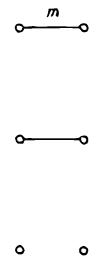
\includegraphics[keepaspectratio]{images/part001_5ff7a109.jpg}}

if \(m = 3\) ) and by

when \(m = 2\) . *The Coxeter graph of the symmetric group \(\mathfrak{S}_n\) is represented by

\pandocbounded{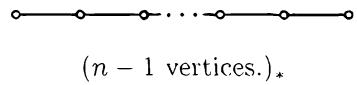
\includegraphics[keepaspectratio]{images/part001_1071b0ee.jpg}}

We show later (Chap. V, §4) that, conversely, any Coxeter matrix is the matrix of a Coxeter system.

A Coxeter system \((W,S)\) is said to be irreducible if the underlying graph of its Coxeter graph is connected (Appendix, no. 2) and non-empty. Equivalently, S is non-empty and there exists no partition of S into two distinct subsets \(S'\) and \(S''\) of S such that every element of \(S'\) commutes with every element of \(S''\) . More generally, let \((\Gamma_{i})_{i\in I}\) be the family of connected components of \(\Gamma\) (Appendix, no. 2) and let \(S_{i}\) be the set of vertices of \(\Gamma_{i}\) . Let \(W_{i}=W_{S_i}\) , be the subgroup of W generated by \(S_{i}\) (cf.~no. 8). Then the \((W_{i},S_{i})\) are irreducible Coxeter systems (no. 8, Th. 2) called the irreducible components of \((W,S)\) . Moreover, the group W is the restricted direct product \(^{4}\) of the subgroups \(W_{i}\) for \(i\in I\) . Indeed, this follows from the following more general proposition:

PROPOSITION 8. Let \((\mathrm{S}_{i})_{i\in\mathrm{I}}\) be a partition of S such that every element of \(S_{i}\) commutes with every element of \(S_{j}\) if \(i\neq j\) . For all \(i\in I\) , let \(W_{i}\) be the subgroup generated by \(S_{i}\) . Then W is the restricted direct product of the family \((\mathrm{W}_{i})_{i\in\mathrm{I}}\) .

It is clear that for all \(i \in I\) the subgroup \(W_i'\) generated by the union of the \(W_j\) for \(j \neq i\) is also generated by \(S_i' = \bigcup_{i \neq j} S_j\) . Thus

\[
\mathrm{W} _ {i} \cap \mathrm{W} _ {i} ^ {\prime} = \mathrm{W} _ {\varnothing} = \{1 \}
\]

by Th. 2 of no. 8. Since W is generated by the union of the \(W_{i}\) , this proves the proposition.

\section{TITS SYSTEMS}

In this paragraph, the letters G, B, N, S, T, W have the meaning indicated in no. 1 below.

\subsection{DEFINITIONS AND FIRST PROPERTIES}

Let G be a group and B a subgroup of G. The group \(B \times B\) acts on G by \((b, b')\) . \(g = bgb'^{-1}\) for \(b, b' \in B\) and \(g \in G\) . The orbits of \(B \times B\) on G are the sets BgB for \(g \in G\) , and are called the double cosets of G with respect to B. They form a partition of G; the corresponding quotient is denoted by B\textbackslash G/B. If C and C' are double cosets, CC' is a union of double cosets.

DEFINITION 1. A Tits system is a quadruple \((\mathbf{G},\mathbf{B},\mathbf{N},\mathbf{S})\) , where \(\mathbf{G}\) is a group, \(\mathbf{B}\) and \(\mathbf{N}\) are two subgroups of \(\mathbf{G}\) and \(\mathbf{S}\) is a subset of \(\mathrm{N} / (\mathrm{B}\cap \mathrm{N})\) , satisfying the following axioms:

(T1) The set \(\mathrm{B} \cup \mathrm{N}\) generates \(\mathrm{G}\) and \(\mathrm{B} \cap \mathrm{N}\) is a normal subgroup of \(\mathrm{N}\) .

(T2) The set S generates the group \(W = N/(B \cap N)\) and consists of elements of order 2.

(T3) \(sBw \subset BwB \cup BswB\) for \(s \in S\) and \(w \in W\) .

(T4) For all \(s \in S\) , \(sBs \not\subset B\) .

The group \(W = N / (B \cap N)\) is sometimes called the Weyl group of the Tits system \((G, B, N, S)\) .

Remarks. 1) We shall see in no. 5 (Cor. of Th. 3) that, if (G, B, N) is given, there exists at most one subset S of N/(B∩N) such that (G, B, N, S) is a Tits system.

\begin{enumerate}
\def\labelenumi{\arabic{enumi})}
\setcounter{enumi}{1}
\tightlist
\item
  Let \((G, B, N, S)\) be a Tits system, and let Z be a normal subgroup of G contained in B. Let \(G' = G/Z, B' = B/Z, N' = N/(Z \cap N)\) , and let \(S'\) be the image of S in \(N'/(B' \cap N')\) . Then one sees immediately that \((G', B', N', S')\) is a Tits system.
\end{enumerate}

Throughout this paragraph, with \((\mathrm{G},\mathrm{B},\mathrm{N},\mathrm{S})\) denoting a Tits system, we set \(T=B\cap N\) and W=N/T. A double coset means a double coset of G with respect to B. For any \(w\in W\) , we set \(C(w)=BwB\) ; this is a double coset.

We are going to deduce several elementary consequences of the axioms (T1) to (T4). We denote by \(w, w', \ldots\) elements of W and by \(s, s', \ldots\) elements of S. The following relations are clear:

\[
\mathrm{C} (1) = \mathrm{B}, \quad \mathrm{C} (w w ^ {\prime}) \subset \mathrm{C} (w). \mathrm{C} (w ^ {\prime}), \quad \mathrm{C} (w ^ {- 1}) = \mathrm{C} (w) ^ {- 1}.\tag{1}
\]

Axiom (T3) can also be written in the form

\[
\mathrm{C} (s). \mathrm{C} (w) \subset \mathrm{C} (w) \cup \mathrm{C} (s w).\tag{2}
\]

Moreover, since \(C(sw) \subset C(s).C(w)\) by (1) and since \(C(s).C(w)\) is a union of double cosets, there are only two possibilities:

\[
\mathrm{C} (s). \mathrm{C} (w) = \left\{ \begin{array}{l l} \mathrm{C} (s w) & \text {if} \mathrm{C} (w) \not \subset \mathrm{C} (s). \mathrm{C} (w) \\ \mathrm{C} (w) \cup \mathrm{C} (s w) & \text {if} \mathrm{C} (w) \subset \mathrm{C} (s). \mathrm{C} (w). \end{array} \right.\tag{3}
\]

By (T4), \(\mathrm{B} \neq \mathrm{C}(s). \mathrm{C}(s)\) ; putting \(w = s\) in (3) and using the relation \(s^2 = 1\) , we obtain

\[
\mathrm{C} (s). \mathrm{C} (s) = \mathrm{B} \cup \mathrm{C} (s).\tag{4}
\]

This formula shows that \(B \cup C(s)\) is a subgroup of G. Multiplying both sides of (4) on the right by \(C(w)\) , and using formula (3) and the relation

\[
\mathrm{B.C} (w) = \mathrm{C} (w),
\]

we obtain

\[
\mathrm{C} (s). \mathrm{C} (s). \mathrm{C} (w) = \mathrm{C} (w) \cup \mathrm{C} (s w).\tag{5}
\]

Taking the inverses of the sets entering into formulas (2), (3) and (5) and then replacing w by \(w^{-1}\) , we obtain the formulas

\[
\mathrm{C} (w). \mathrm{C} (s) \subset \mathrm{C} (w) \cup \mathrm{C} (w s)\tag{(2')}
\]

\[
\mathrm{C} (w). \mathrm{C} (s) = \mathrm{C} (w s) \quad \text {   if   } \mathrm{C} (w) \not \subset \mathrm{C} (w). \mathrm{C} (s)
\]

\[
\mathrm{C} (w). \mathrm{C} (s) = \left\{ \begin{array}{l l} \mathrm{C} (w) \cup \mathrm{C} (w s) & \text {if} \mathrm{C} (w) \subset \mathrm{C} (w). \mathrm{C} (s) \end{array} \right.\tag{3'}
\]

\[
\mathrm{C} (w). \mathrm{C} (s). \mathrm{C} (s) = \mathrm{C} (w) \cup \mathrm{C} (w s).\tag{(5')}
\]

Lemma 1. Let \(s_1, \ldots, s_q \in S\) and let \(w \in W\) . We have

\[
\mathrm{C} \left(s _ {1} \dots s _ {q}\right). \mathrm{C} (w) \subset \bigcup_ {\left(i _ {1}, \dots i _ {p}\right)} \mathrm{C} \left(s _ {i _ {1}} \dots s _ {i _ {p}} w\right),
\]

where \((i_1, \ldots, i_p)\) denotes the set of strictly increasing sequences of integers in the interval \([1, q]\) .

We argue by induction on \(q\) , the case \(q = 0\) being trivial. If \(q \geqslant 1\) , we have \(C(s_1 \ldots s_q).C(w) \subset C(s_1).C(s_2 \ldots s_q).C(w)\) . By the induction hypothesis, \(C(s_2 \ldots s_q).C(w)\) is contained in the union of the \(C(s_{j_1} \ldots s_{j_p}w)\) , where

\[
2 \leqslant j _ {1} <   \dots <   j _ {p} \leqslant q.
\]

By (T3), the set \(C(s_{1}).C(s_{j_{1}}\ldots s_{j_{p}}w)\) is contained in the union of the sets \(C(s_{1}s_{j_{1}}\ldots s_{j_{p}}w)\) and \(C(s_{j_{1}}\ldots s_{j_{p}}w)\) . This proves the lemma.

\subsection{AN EXAMPLE}

Let \(k\) be a field, \(n\) an integer \(\geqslant 0\) , and \((e_i)\) the canonical basis of \(k^n\) . Let \(G = GL(n, k)\) , let \(B\) be the upper triangular subgroup of \(G\) , and let \(N\) be the subgroup of \(G\) consisting of the matrices having exactly one non-zero element in each row and column. An element of \(N\) permutes the lines \(ke_i\) ; this gives rise to a surjective homomorphism \(N \to \mathfrak{S}_n\) whose kernel is the subgroup \(T = B \cap N\) of diagonal matrices, and allows us to identify \(W = N/T\) with \(\mathfrak{S}_n\) . We denote by \(s_j\) ( \(1 \leqslant j \leqslant n - 1\) ) the element of \(W\) corresponding to the transposition of \(j\) and \(j + 1\) ; let \(S\) be the set of \(s_j\) . The quadruple \((G, B, N, S)\) is a Tits system. Indeed:

Axiom (T1) follows from Cor. 2 of Prop. 14 of Algebra, Chap. II, § 10, no. 13.

Axiom (T2) is proved in Algebra, Chap. I, Correction to p.~97.

Axiom (T4) is immediate.

It remains to verify axiom (T3), i.e.

\[
s _ {j} \mathrm{B} w \subset \mathrm{B} w \mathrm{B} \cup \mathrm{B} s _ {j} w \mathrm{B} \quad \text { for } 1 \leqslant j \leqslant n - 1, w \in \mathrm{W},
\]

or equivalently,

\[
s _ {j} \mathrm{B} \subset \mathrm{BB} ^ {\prime} \cup \mathrm{Bs} _ {j} \mathrm{B} ^ {\prime}, \quad \text { with } \mathrm{B} ^ {\prime} = w \mathrm{B} w ^ {- 1}.
\]

Let \(G_{j}\) be the subgroup of G consisting of the elements that fix the \(e_{i}\) for \(i \neq j, j + 1\) and stabilize the plane spanned by \(e_{j}\) and \(e_{j+1}\) ; this group is isomorphic to \(\mathbf{GL}(2, k)\) . One checks that \(G_{j}B = BG_{j}\) . Since \(s_{j} \in G_{j}\) , we have \(s_{j}B \subset BG_{j}\) , and it suffices to prove that

\[
\mathrm{G} _ {j} \subset (\mathrm{B} \cap \mathrm{G} _ {j}) (\mathrm{B} ^ {\prime} \cap \mathrm{G} _ {j}) \cup (\mathrm{B} \cap \mathrm{G} _ {j}) s _ {j} (\mathrm{B} ^ {\prime} \cap \mathrm{G} _ {j}).
\]

Identify \(G_{j}\) with \(\mathbf{GL}(2,k)\) ; the group \(B \cap G_{j}\) is then identified with the upper triangular subgroup \(B_{2}\) of \(\mathbf{GL}(2,k)\) , while the group \(B' \cap G_{j}\) is identified with \(\mathbf{B}_2\) when \(w(j) < w(j + 1)\) and with the lower triangular subgroup \(\mathbf{B}_2^-\) otherwise. In the first case, the formula to be proved can be written

\[
\mathbf {G L} (2, k) = \mathrm{B} _ {2} \cup \mathrm{B} _ {2} s \mathrm{B} _ {2} \quad \text { where } \quad s = \left( \begin{array}{c c} 0 & 1 \\ 1 & 0 \end{array} \right);
\]

this follows for example from the fact that \(B_{2}\) is the stabilizer of a point for the action of \(\mathbf{GL}(2,k)\) on the projective line \(\mathbf{P}_{1}(k)\) , and acts transitively on the complement of this point. In the second case, the formula to be proved can be written

\[
\mathbf {G L} (2, k) = \mathrm{B} _ {2} \mathrm{B} _ {2} ^ {-} \cup \mathrm{B} _ {2} s \mathrm{B} _ {2} ^ {-};
\]

since \(B_{2}^{-} = sB_{2}s\) , this follows from the preceding formula by multiplying on the right by s.

\subsection{DECOMPOSITION OF G INTO DOUBLE COSETS}

THEOREM 1. We have G = BWB. The map \(w \mapsto C(w)\) is a bijection from W to the set B\textbackslash G/B of double cosets of G with respect to B.

It is clear that BWB is stable under \(x \mapsto x^{-1}\) , and Lemma 1 shows that it is stable under the product. Since it contains B and N, it is equal to G.

It remains to prove that \(\mathrm{C}(w) \neq \mathrm{C}(w')\) if \(w \neq w'\) . For this, we shall prove by induction on the integer \(q\) the following assertion:

(Aq) If w and \(w'\) are distinct elements of W such that \(l_{S}(w) \geqslant l_{S}(w') = q\) , then \(C(w) \neq C(w')\) .

(For the definition of \(l_{\mathbb{S}}(w)\) , see §1, no. 1.)

This assertion is clear for \(q = 0\) , since then \(w' = 1\) and \(w \neq 1\) , hence \(C(w') = B\) and \(C(w) \neq B\) .

Assume that \(q \geqslant 1\) and that \(w, w'\) satisfy the hypotheses of \((\mathbf{A}_q)\) . There exists \(s \in S\) such that \(sw'\) is of length \(q - 1\) . We have

\[
l _ {S} (w) > l _ {S} \left(s w ^ {\prime}\right)\tag{6}
\]

hence \(w \neq sw'\) . Moreover, \(sw \neq sw'\) ; by formula (3) of §1, no. 1, we have

\[
l _ {\mathrm{S}} (s w) \geqslant l _ {\mathrm{S}} (w) - 1 \geqslant l _ {\mathrm{S}} (s w ^ {\prime}) = q - 1.\tag{7}
\]

By the induction hypothesis, \(C(sw')\) is distinct from \(C(w)\) and from \(C(sw)\) ; from formula (2) it follows that

\[
\mathrm{C} (s w ^ {\prime}) \cap \mathrm{C} (s). \mathrm{C} (w) = \varnothing .\tag{8}
\]

Since \(\mathrm{C}(sw') \subset \mathrm{C}(s).\mathrm{C}(w')\) , we have finally that \(\mathrm{C}(w) \neq \mathrm{C}(w')\) .

Remark. Axiom (T4) was not used in the preceding proof.

\subsection{RELATIONS WITH COXETER SYSTEMS}

THEOREM 2. The pair \((\mathrm{W},\mathrm{S})\) is a Coxeter system. Moreover, for \(s\in \mathrm{S}\) and \(w\in \mathrm{W}\) , the relations \(\mathrm{C}(sw) = \mathrm{C}(s).C(w)\) and \(l_{\mathbb{S}}(sw) > l_{\mathbb{S}}(w)\) are equivalent.

For any \(s \in S\) , let \(P_s\) be the set of elements \(w \in W\) such that

\[
\mathrm{C} (s). \mathrm{C} (w) = \mathrm{C} (s w).
\]

We are going to verify that the \(P_{s}\) satisfy conditions ( \(A'\) ), ( \(B'\) ) and (C) of §1, no. 7; the two assertions of the theorem will then follow from Prop. 6 of §1, no. 7.

Condition \((\mathbf{A}^{\prime})\) is clear.

We verify (B'). If \(P_{s}\) and \(sP_{s}\) had an element w in common, we would have \(w \in P_{s}\) and \(sw \in P_{s}\) , and hence

\[
\mathrm{C} (s). \mathrm{C} (w) = \mathrm{C} (s w), \quad \mathrm{C} (s). \mathrm{C} (s w) = \mathrm{C} (w).
\]

It would follow that \(\mathrm{C}(s).\mathrm{C}(s).\mathrm{C}(w) = \mathrm{C}(w)\) and, by formula (5), this would imply that \(\mathrm{C}(w) = \mathrm{C}(sw)\) , which would contradict Th. 1.

We verify (C). Let \(s, s' \in S\) and \(w, w' \in W\) with \(w' = ws'\) . The assumption that \(w \in P_s\) and \(w' \notin P_s\) implies that

\[
\mathrm{C} (s w) = \mathrm{C} (s). \mathrm{C} (w)\tag{9}
\]

\[
\mathrm{C} (w ^ {\prime}) \subset \mathrm{C} (s). \mathrm{C} (w ^ {\prime})\tag{10}
\]

by (3).

From (9) and the relation \(w = w's'\) , it follows that

\[
\mathrm{C} (s) w ^ {\prime} s ^ {\prime} \mathrm{B} = \mathrm{C} (s w).\tag{11}
\]

By formula \((2')\) , \(C(w')\) . \(C(s') \subset C(w') \cup C(w's')\) , which immediately implies that

\[
\mathrm{C} (w ^ {\prime}) s ^ {\prime} \mathrm{B} \subset \mathrm{C} (w s ^ {\prime}) \cup \mathrm{C} (w).\tag{12}
\]

Since \(C(w')\) is a union of left cosets gB and since

\[
\mathrm{C} (s). \mathrm{C} (w ^ {\prime}) = \mathrm{C} (s) w ^ {\prime} \mathrm{B},
\]

formula (10) shows that \(C(s)w'\) meets \(C(w')\) and a fortiori that \(C(s)w's'B\) meets \(C(w')s'B\) . It follows from formulas (11) and (12) that the double coset \(C(sw)\) is equal to one of the double cosets \(C(ws')\) and \(C(w)\) ; since \(sw \neq w\) , Th. 1 allows us to conclude that \(sw = ws'\) .

COROLLARY 1. Let \(w_{1}, \ldots, w_{q} \in \mathbf{W}\) and let \(w = w_{1} \ldots w_{q}\) . If

\[
l _ {S} (w) = l _ {S} \left(w _ {1}\right) + \dots + l _ {S} \left(w _ {q}\right),
\]

then

\[
\mathrm{C} (w) = \mathrm{C} (w _ {1}) \dots \mathrm{C} (w _ {q}).
\]

On taking reduced decompositions of the \(w_{i}\) , one is reduced to the case of a reduced decomposition

\[
w = s _ {1} \dots s _ {q}, \quad \text { with } s _ {i} \in S.
\]

If \(u = s_2 \ldots s_q\) , then \(w = s_1u\) and \(l_{\mathbb{S}}(s_1u) > l_{\mathbb{S}}(u)\) , so \(\mathrm{C}(w) = \mathrm{C}(s_1). \mathrm{C}(u)\) by the theorem. The required formula follows from this by induction on \(q\) .

COROLLARY 2. Let \(w \in W\) and let \(T_w\) be the subset of \(W\) associated to \(w\) by the procedure of Lemma 2 of § 1, no. 4. If \(t \in T_w\) , then

\[
\mathrm{C} (t) \subset \mathrm{C} (w). \mathrm{C} (w ^ {- 1}).
\]

If \(t \in \mathrm{T}_w\) , there exist by definition elements \(w', w'' \in \mathrm{W}\) and \(s \in \mathrm{S}\) such that

\[
w = w ^ {\prime} s w ^ {\prime \prime}, l _ {S} (w) = l _ {S} (w ^ {\prime}) + l _ {S} (w ^ {\prime \prime}) + 1 \quad \text {and} \quad t = w ^ {\prime} s w ^ {\prime - 1}.
\]

By Cor. 1,

\[
\mathrm{C} (w). \mathrm{C} (w ^ {- 1}) = \mathrm{C} (w ^ {\prime}). \mathrm{C} (s). \mathrm{C} (w ^ {\prime \prime}). \mathrm{C} (w ^ {\prime \prime - 1}). \mathrm{C} (s). \mathrm{C} (w ^ {\prime - 1}).
\]

Hence,

\[
\mathrm{C} (w). \mathrm{C} (w ^ {- 1}) \supset \mathrm{C} (w ^ {\prime}). \mathrm{C} (s). \mathrm{C} (s). \mathrm{C} (w ^ {\prime - 1}).
\]

By (4), \(\mathrm{C}(s) \subset \mathrm{C}(s). \mathrm{C}(s)\) . Hence,

\[
\mathrm{C} (w). \mathrm{C} (w ^ {- 1}) \supset \mathrm{C} (w ^ {\prime}). \mathrm{C} (s). \mathrm{C} (w ^ {\prime - 1}) \supset \mathrm{C} (t).
\]

COROLLARY 3. Let \(w \in W\) and let \(H_w\) be the subgroup of \(G\) generated by \(C(w).C(w^{-1})\) . Then:

\begin{enumerate}
\def\labelenumi{\alph{enumi})}
\tightlist
\item
  For any reduced decomposition \((s_1,\ldots ,s_q)\) of \(w\) ,
\end{enumerate}

\[
\mathrm{C} (s _ {j}) \subset \mathrm{H} _ {w} \quad \text { for } 1 \leqslant j \leqslant q.
\]

\begin{enumerate}
\def\labelenumi{\alph{enumi})}
\setcounter{enumi}{1}
\tightlist
\item
  The group \(\mathrm{H}_w\) contains \(\mathrm{C}(w)\) and is generated by \(\mathrm{C}(w)\) .
\end{enumerate}

We prove \(a)\) by induction on \(j\) . Assume that \(C(s_k)\) is contained in \(H_w\) for \(k < j\) . Let

\[
t = (s _ {1} \dots s _ {j - 1}) s _ {j} (s _ {1} \dots s _ {j - 1}) ^ {- 1}.
\]

The element \(t\) belongs to the subset \(\mathrm{T}_w\) of \(\mathbf{W}\) defined in Lemma 2 of §1, no. 4. By Cor. 2, \(\mathrm{C}(t) \subset \mathrm{H}_w\) , and hence \(\mathrm{C}(s_j) \subset \mathrm{H}_w\) .

Since \(\mathrm{C}(w) = \mathrm{C}(s_1) \ldots \mathrm{C}(s_q)\) , cf.~Cor. 1, we have \(\mathrm{C}(w) \subset \mathrm{H}_w\) , and \(b)\) follows.

Example. Th. 2, applied to the Tits system described in no. 2, shows that the symmetric group \(S_{n}\) , with the set of transpositions of consecutive elements, is a Coxeter group.

\subsection{SUBGROUPS OF G CONTAINING B}

For any subset \(X\) of \(S\) , we denote by \(W_X\) the subgroup of \(W\) generated by \(X\) (cf.~§1, no. 8) and by \(G_X\) the union \(BW_X B\) of the double cosets \(C(w)\) , \(w \in W_X\) . We have \(G_\varnothing = B\) and \(G_S = G\) .

THEOREM 3. a) For any subset \(X\) of \(S\) , the set \(G_X\) is a subgroup of \(G\) , generated by \(\bigcup_{s \in X} C(s)\) .

\begin{enumerate}
\def\labelenumi{\alph{enumi})}
\setcounter{enumi}{1}
\item
  The map \(\mathrm{X} \mapsto \mathrm{G}_{\mathrm{X}}\) is a bijection from \(\mathfrak{P}(\mathrm{S})\) to the set of subgroups of \(\mathrm{G}\) containing \(\mathrm{B}\) .
\item
  Let \((\mathrm{X}_i)_{i\in I}\) be a family of subsets of X. If \(X = \bigcap_{i\in I}X_i\) , then \(G_X = \bigcap_{i\in I}G_{X_i}\) .
\item
  Let X and Y be two subsets of S. Then \(G_{X} \subset G_{Y}\) (resp. \(G_{X} = G_{Y}\) ) if and only if \(X \subset Y\) (resp. X = Y).
\end{enumerate}

It is clear that \(G_{X} = (G_{X})^{-1}\) ; Lemma 1 of no. 1 shows that \(G_{X}.G_{X} \subset G_{X}\) ; and hence \(a)\) follows, taking into account Cor. 1 of Th. 2.

The injectivity of \(\mathrm{X} \mapsto \mathrm{G}_{\mathrm{X}}\) follows from that of \(\mathrm{X} \mapsto \mathrm{W}_{\mathrm{X}}\) (§1, no. 8, Th. 2). Conversely, let \(\mathrm{H}\) be a subgroup of \(\mathrm{G}\) containing \(\mathrm{B}\) . Let \(\mathrm{U}\) be the set of \(w \in \mathrm{W}\) such that \(C(w) \subset \mathrm{H}\) . We have \(\mathrm{H} = \mathrm{BUB}\) since \(\mathrm{H}\) is a union of double cosets. Let \(\mathrm{X} = \mathrm{U} \cap \mathrm{S}\) ; we show that \(\mathrm{H} = \mathrm{G}_{\mathrm{X}}\) . Clearly, \(\mathrm{G}_{\mathrm{X}} \subset \mathrm{H}\) . On the other hand, let \(u \in \mathrm{U}\) and let \((s_1, \ldots, s_q)\) be a reduced decomposition of \(u\) . Cor. 3 of Th. 2 implies that \(C(s_j) \subset \mathrm{H}\) , and hence that \(s_j \in \mathrm{X}\) for \(1 \leqslant j \leqslant q\) . Thus, \(u \in \mathrm{W}_{\mathrm{X}}\) , and since \(\mathrm{H}\) is the union of the \(C(u)\) for \(u \in \mathrm{U}\) , we have \(\mathrm{H} \subset \mathrm{G}_{\mathrm{X}}\) , which proves \(b\) ).

Assertions \(c)\) and \(d)\) follow from analogous properties of \(W_X\) ( \(\S 1\) , no. 8, Th. 2).

COROLLARY. The set \(S\) consists of the elements \(w \in W\) such that \(w \neq 1\) and \(B \cup C(w)\) is a subgroup of \(G\) .

The elements \(w \in W\) such that \(B \cup C(w)\) is a subgroup of G are those for which there exists \(X \subset S\) with \(W_{X} = \{1, w\}\) . Moreover, if \(w \neq 1\) , we necessarily have \(\text{Card}(X) = 1\) , i.e.~\(w \in S\) .

Remark. 1) The above corollary shows that S is determined by (G, B, N); for this reason, we sometimes allow ourselves to say that (G, B, N) is a Tits system, or that (B, N) is a Tits system in G.

PROPOSITION 1. Let X be a subset of S and N' a subgroup of N whose image in W is equal to W\_X. Then, (G\_X, B, N', X) is a Tits system.

We have \(G_{X} = BW_{X}B = BN'B\) , which shows that \(G_{X}\) is generated by \(B \cup N'\) . The verification of the axioms (T1) to (T4) is now immediate.

PROPOSITION 2. Let \(\mathrm{X}, \mathrm{Y} \subset \mathrm{S}\) and \(w \in \mathrm{W}\) . We have

\[
\mathrm{G} _ {\mathrm{X}} w \mathrm{G} _ {\mathrm{Y}} = \mathrm{BW} _ {\mathrm{X}} w \mathrm{W} _ {\mathrm{Y}} \mathrm{B}.
\]

Let \(s_1, \ldots, s_q \in X\) and \(t_1, \ldots, t_q \in Y\) . Lemma 1 shows that

\[
\mathrm{C} (s _ {1} \dots s _ {q}). \mathrm{C} (w). \mathrm{C} (t _ {1} \dots t _ {q}) \subset \mathrm{BW} _ {\mathrm{X}} w \mathrm{W} _ {\mathrm{Y}} \mathrm{B},
\]

and hence that

\[
\mathrm{G} _ {\mathrm{X}} w \mathrm{G} _ {\mathrm{Y}} \subset \mathrm{BW} _ {\mathrm{X}} w \mathrm{W} _ {\mathrm{Y}} \mathrm{B}.
\]

The opposite inclusion is obvious.

Remark. 2) Denote by \(G_X \backslash G / G_Y\) the set of subsets of \(G\) of the form \(G_X gG_Y\) , \(g \in G\) ; and define \(W_X \backslash W / W_Y\) analogously. The preceding proposition shows that the canonical bijection \(w \mapsto C(w)\) from \(W\) to \(B \backslash G / B\) defines by passage to the quotient a bijection \(W_X \backslash W / W_Y \to G_X \backslash G / G_Y\) .

PROPOSITION 3. Let \(\mathbf{X} \subset \mathbf{S}\) and \(g \in \mathbf{G}\) . The relation \(g\mathrm{B}g^{-1} \subset \mathbf{G}_{\mathbf{X}}\) implies that \(g \in \mathbf{G}_{\mathbf{X}}\) .

Let \(w \in W\) be such that \(g \in C(w)\) . Since B is a subgroup of \(G_X\) , the hypothesis \(gBg^{-1} \subset G_X\) implies that \(C(w).C(w^{-1}) \subset G_X\) , and hence that \(C(w) \subset G_X\) by Cor. 3 of Th. 2, so g belongs to \(G_X\) .

\subsection{PARABOLIC SUBGROUPS}

DEFINITION 2. A subgroup of G is said to be parabolic if it contains a conjugate of B.

It is clear that every subgroup that contains a parabolic subgroup is parabolic.

PROPOSITION 4. Let P be a subgroup of G.

\begin{enumerate}
\def\labelenumi{\alph{enumi})}
\item
  P is parabolic if and only if there exists a subset X of S such that P is conjugate to \(G_{X}\) (cf.~no. 5 for the definition of \(G_{X}\) ).
\item
  Let \(\mathrm{X}, \mathrm{X}' \subset \mathrm{S}\) and \(g, g' \in \mathrm{G}\) be such that \(\mathrm{P} = g\mathrm{G}_{\mathrm{X}}g^{-1} = g'\mathrm{G}_{\mathrm{X}'}g'^{-1}\) . Then, \(\mathrm{X} = \mathrm{X}'\) and \(g'g^{-1} \in \mathrm{P}\) .
\end{enumerate}

Assertion a) follows from Th. 3, b).

Under the hypotheses of \(b\) ), we have

\[
g ^ {- 1} g ^ {\prime} \mathrm{B} g ^ {\prime - 1} g \subset g ^ {- 1} g ^ {\prime} \mathrm{G} _ {\mathrm{X} ^ {\prime}} g ^ {\prime - 1} g = \mathrm{G} _ {\mathrm{X}},
\]

and Prop. 3 shows that \(g^{-1}g' \in \mathrm{G}_X\) . Hence, \(\mathrm{G}_{\mathrm{X}'} = \mathrm{G}_X\) and \(\mathrm{X}' = \mathrm{X}\) by Th. 3, b). Finally,

\[
g ^ {\prime} g ^ {- 1} = g. g ^ {- 1} g ^ {\prime}. g ^ {- 1} \in g \mathrm{G} _ {\mathrm{X}} g ^ {- 1},
\]

which proves b).

If the parabolic subgroup P is conjugate to \(G_{X}\) , where \(X \subset S\) , then P is said to be of type X.

THEOREM 4. (i) Let \(\mathbf{P}_1\) and \(\mathbf{P}_2\) be two parabolic subgroups of \(\mathbf{G}\) whose intersection is parabolic and let \(g \in \mathbf{G}\) be such that \(g\mathrm{P}_1g^{-1} \subset \mathrm{P}_2\) . Then \(g \in \mathbf{P}_2\) and \(\mathbf{P}_1 \subset \mathbf{P}_2\) .

\begin{enumerate}
\def\labelenumi{(\roman{enumi})}
\setcounter{enumi}{1}
\item
  Two parabolic subgroups whose intersection is parabolic are not conjugate.
\item
  Let \(\mathbf{Q}_1\) and \(\mathbf{Q}_2\) be two parabolic subgroups of \(\mathbf{G}\) contained in a subgroup \(\mathbf{Q}\) of \(\mathbf{G}\) . Then any \(g \in \mathbf{G}\) such that \(g\mathbf{Q}_1g^{-1} = \mathbf{Q}_2\) belongs to \(\mathbf{Q}\) .
\item
  Every parabolic subgroup is its own normaliser \(^{6}\) .
\end{enumerate}

Assertion (i) follows from Props. 3 and 4, and implies (ii). Under the hypotheses of (iii), we have \(gQ_{1}g^{-1} \subset Q\) , which implies that \(g \in Q\) by (i). Finally, (iv) follows from (iii) by taking \(Q_{1} = Q_{2} = Q\) .

PROPOSITION 5. Let \(\mathbf{P}_1\) and \(\mathbf{P}_2\) be two parabolic subgroups of \(\mathbf{G}\) . Then \(\mathbf{P}_1 \cap \mathbf{P}_2\) contains a conjugate of \(\mathbf{T}\) .

By first transforming \(P_{1}\) and \(P_{2}\) by an inner automorphism of G, we may assume that \(B \subset P_{1}\) . Let \(g \in G\) be such that \(gBg^{-1} \subset P_{2}\) . By Th. 1, there exist \(n \in N\) and \(b, b' \in B\) such that \(g = bnb'\) . Since T is normal in N,

\[
\mathrm{P} _ {2} \supset g \mathrm{B} g ^ {- 1} = b n \mathrm{B} n ^ {- 1} b ^ {- 1} \supset b n \mathrm{T} n ^ {- 1} b ^ {- 1} = b \mathrm{T} b ^ {- 1}
\]

and

\[
\mathrm{P} _ {1} \supset \mathrm{B} \supset b \mathrm{T} b ^ {- 1},
\]

which proves the proposition.

\subsection{SIMPLICITY THEOREMS}

Lemma 2. Let H be a normal subgroup of G. There exists a subset X of S such that BH = G\_X and such that every element of X commutes with every element of S-X.

Since BH is a subgroup of G containing B, there exists a unique subset X of S such that \(BH = G_{X}\) (Th. 3).

Let \(s_1 \in X\) and \(s_2 \in S - X\) ; let \(n_1\) and \(n_2\) be representatives in \(N\) of \(s_1\) and \(s_2\) , respectively. Then \(n_1 \in G_X = BH\) and there exists \(b \in B\) such that \(bn_1 \in H\) . Since \(H\) is normal in \(G\) , the element \(h = n_2bn_1n_2^{-1}\) of \(G\) belongs to \(H\) . This means that

\[
h \in \mathrm{C} (s _ {2}). \mathrm{C} (s _ {1}). \mathrm{C} (s _ {2}).
\]

If the length of \(s_2s_1s_2\) is equal to 3, Cor. 1 of Th. 2 implies that

\[
\mathrm{C} (s _ {2}). \mathrm{C} (s _ {1}). \mathrm{C} (s _ {2}) = \mathrm{C} (s _ {2} s _ {1} s _ {2}),
\]

and hence that \(h \in H \cap C(s_{2}s_{1}s_{2})\) . Since \(H \cap C(s_{2}s_{1}s_{2})\) is non-empty, \(s_{2}s_{1}s_{2} \in W_{X}\) . As \((s_{2}, s_{1}, s_{2})\) is a reduced decomposition, it follows that \(s_{2} \in X\) , contrary to our assumption.

Thus \(l_{\mathrm{S}}(s_2s_1s_2) \leqslant 2\) ; if \(l_{\mathrm{S}}(s_2s_1s_2) = 1\) , then \(s_1s_2 \in \mathrm{S}\) and so \((s_1s_2)^2 = 1\) , or \(s_1s_2 = s_2s_1\) . If \(l_{\mathrm{S}}(s_2s_1s_2) = 2\) , property (E) of §1, no. 5 implies that \(s_2s_1 = s_1s_2\) , since \(s_1 \neq s_2\) . Q.E.D.

The following property of a group U enters into Th. 5 below:

\begin{enumerate}
\def\labelenumi{(\Alph{enumi})}
\setcounter{enumi}{17}
\tightlist
\item
  For any normal subgroup V of U distinct from U, the commutator subgroup (cf.~Algebra, Chap. I, §6, no. 8) of U/V is distinct from U/V.
\end{enumerate}

Every soluble group satisfies (R); in particular, every abelian group satisfies (R). It can be shown that the symmetric group \(S_{n}\) satisfies (R) (cf.~Exerc. 29).

THEOREM 5. Let Z be the intersection of the conjugates of B, let U be a subgroup of B and let \(G_{1}\) be the subgroup generated by the conjugates of U in G. We make the following assumptions:

\begin{enumerate}
\def\labelenumi{(\arabic{enumi})}
\item
  U is normal in B and B = UT.
\item
  U has property (R.).
\item
  \(\mathbf{G}_1\) is equal to its commutator subgroup.
\item
  The Coxeter system (W, S) is irreducible (cf.~§ 1, no. 9).
\end{enumerate}

Then every subgroup H of G normalised by \(G_{1}\) is either contained in Z or contains \(G_{1}\) .

First we show that \(G = G_{1}T\) . The group \(G_{1}T\) contains B and hence is its own normaliser (Th. 4); but as N normalises \(G_{1}\) and T, it also normalises \(G_{1}T\) , so \(N \subset G_{1}T\) . Since G is generated by B and N, it follows that \(G = G_{1}T\) .

Next, set

\[
\begin{array}{c} \mathrm{G} ^ {\prime} = \mathrm{G} _ {1} \mathrm{H}, \quad \mathrm{B} ^ {\prime} = \mathrm{B} \cap \mathrm{G} ^ {\prime}, \quad \mathrm{N} ^ {\prime} = \mathrm{N} \cap \mathrm{G} ^ {\prime}, \\ \mathrm{T} ^ {\prime} = \mathrm{T} \cap \mathrm{G} ^ {\prime} = \mathrm{B} ^ {\prime} \cap \mathrm{N} ^ {\prime} \quad \text {and} \quad \mathrm{W} ^ {\prime} = \mathrm{N} ^ {\prime} / \mathrm{T} ^ {\prime}. \end{array}
\]

We have \(G = G'T\) since \(G'\) contains \(G_{1}\) , and hence \(N = N'T\) . The inclusion of \(N'\) into N thus defines, on passing to the quotient, an isomorphism \(\alpha : W' \to W\) . Let \(S' = \alpha^{-1}(S)\) .

We now show that \((\mathrm{G}^{\prime},\mathrm{B}^{\prime},\mathrm{N}^{\prime},\mathrm{S}^{\prime})\) is a Tits system. Since G = BNB and B = TU = UT, we have G = UNU. Since U is a subgroup of \(G^{\prime}\) , it follows that \(G^{\prime} = UN^{\prime}U\) ; since \(U \subset B^{\prime}\) , this proves (T1). Axiom (T2) is satisfied since \(\alpha\) is an isomorphism. Let \(w \in W\) and let \(w' = \alpha^{-1}(w)\) be the corresponding element of \(W^{\prime}\) . We have

\[
\mathrm{B} w \mathrm{B} = \mathrm{B} w \mathrm{B} ^ {\prime} = \mathrm{B} w ^ {\prime} \mathrm{B} ^ {\prime}, \quad \text { since } \mathrm{B} = \mathrm{B} ^ {\prime} \mathrm{T}.
\]

From this we conclude that \(G' \cap BwB = B'w'B'\) , which means that the inclusion of \(G'\) into G defines on passing to the quotient a bijection from

\(B'\backslash G'/B'\) to \(B\backslash G/B\) . Axiom (T3) follows immediately. Axiom (T4) follows from \(B = B'T\) .

The subgroup H is normal in \(G'\) . By Lemma 2 applied to \((G', B', N', S')\) , there exists a subset \(X'\) of \(S'\) such that \(B'H = G_{X'}'\) and every element of \(S' - X'\) commutes with every element of \(X'\) . In view of assumption (4), there are only two possibilities:

\begin{enumerate}
\def\labelenumi{\alph{enumi})}
\item
  \(X' = \varnothing\) , i.e.~\(B'H = B'\) , so \(H \subset B' \subset B\) . If \(g \in G\) , then \(g = g_1 t\) with \(g_1 \in G_1\) , \(t \in T\) , and \(H \subset g_1 Bg_1^{-1}\) since \(G_1\) normalises \(H\) . Thus \(H \subset gBg^{-1}\) , and since \(Z\) is the intersection of the \(gBg^{-1}\) , we have \(H \subset Z\) .
\item
  \(X' = S'\) , i.e.~\(B'H = G'\) . Since \(G = G'T\) , we have
\end{enumerate}

\[
\mathrm{G} = \mathrm{B} ^ {\prime} \mathrm{HT} = \mathrm{HB} ^ {\prime} \mathrm{T} = \mathrm{HB}.
\]

As B normalises U, every conjugate of U is of the form \(hUh^{-1}\) with \(h \in H\) . Such a subgroup is contained in the group UH, hence \(G_{1} \subset UH\) by the definition of \(G_{1}\) . Thus, we have the isomorphisms

\[
\mathrm{U} / (\mathrm{U} \cap \mathrm{H}) \cong \mathrm{UH} / \mathrm{H} = \mathrm{G} _ {1} \mathrm{H} / \mathrm{H} \cong \mathrm{G} _ {1} / (\mathrm{G} _ {1} \cap \mathrm{H}).
\]

By assumption (3), \(G_{1}/(G_{1} \cap H)\) is equal to its commutator subgroup. Assumption (2) now shows that the group \(U/(U \cap H)\) , which is isomorphic to \(G_{1}/(G_{1} \cap H)\) , reduces to the identity element. Hence \(G_{1} \cap H = G_{1}\) and \(G_{1} \subset H\) , which completes the proof.

COROLLARY. Under the assumptions of Th. 5, the group \(\mathrm{G}_{1}/(\mathrm{G}_{1} \cap \mathrm{Z})\) is either simple non-abelian or reduces to the identity element.

Th. 5 shows that \(G_{1}/(G_{1} \cap Z)\) is simple or reduces to the identity element. On the other hand, assumption (3) implies that it is equal to its commutator subgroup. Hence the corollary.

Remarks. 1) Assumptions (2), (3), (4) were not used in the proof that \((\mathbf{G}', \mathbf{B}', \mathbf{N}', \mathbf{S}')\) is a Tits system.

\begin{enumerate}
\def\labelenumi{\arabic{enumi})}
\setcounter{enumi}{1}
\item
  Suppose that \(\mathbf{Z} \cap \mathbf{U} = \{1\}\) . Since \(\mathbf{Z}\) and \(\mathbf{U}\) are normal in \(\mathbf{B}\) , it follows that every element of \(\mathbf{Z}\) commutes with every element of \(\mathbf{U}\) , and hence with every element of \(\mathbf{G}_1\) . In view of the preceding corollary, it follows that \(\mathbf{G}_1 \cap \mathbf{Z}\) is the centre of \(\mathbf{G}_1\) .
\item
  Assumption (3) is implied by the following condition:
\end{enumerate}

(3') U is generated by the commutators \(b^{-1}u^{-1}bu\) with \(u \in \mathbf{U}\) and \(b \in \mathbf{B} \cap \mathbf{G}_1\) .

Examples. 1) Let \(k\) be a field, \(n\) an integer \(\geqslant 0\) , \(G = \mathbf{GL}(n, k)\) , and let \((G, B, N, S)\) be the Tits system described in no. 2. Let \(U\) be the strictly upper triangular subgroup of \(G\) , i.e.~the subgroup of \(B\) consisting of the matrices whose diagonal entries are equal to 1. Condition (1) in Th. 5 is immediate, and so is (2) since U is soluble. Condition (4) is satisfied if \(n \geqslant 2\) . One can show (cf.~Algebra, Chap. II, §10, Exerc. 13) that (3) is satisfied if \(n \geqslant 3\) and \(\operatorname{Card}(k) \geqslant 4\) . Under these conditions, we conclude that \(G_{1}/(G_{1} \cap Z)\) is simple and that \(G_{1} \cap Z\) is the centre of \(G_{1}\) (cf.~Remark 2).

When \(k\) is commutative, \(G_1 = \mathbf{SL}(n,k)\) (cf.~Algebra, Chap. III, § 8, no. 9).

*2) Let \(\mathfrak{g}\) be a simple Lie algebra over \(\mathbf{C}\) , and let \(\mathbf{G}\) be the group of inner automorphisms of \(\mathfrak{g}\) (cf.~Chap. III, §6, no. 2, Prop. 2). By using Th. 5, one can show that \(\mathbf{G}\) is simple non-abelian.*

\appendixsection{Appendix. Graphs}

\appendixitem{DEFINITIONS}

DEFINITION 1. A combinatorial graph (or simply a graph, if there is no risk of confusion) is a pair \((\mathrm{A},\mathrm{S})\) , where \(\mathrm{S}\) is a set and \(\mathrm{A}\) is a subset of \(\mathfrak{P}(\mathrm{S})\) consisting of sets with two elements.

Let \(\Gamma = (A, S)\) be a graph. The elements of A are called the edges and those of S the vertices of \(\Gamma\) ; two vertices are said to be joined if \(\{x, y\}\) is an edge. A vertex is called terminal if it is joined to at most one vertex, and a ramification point if it is joined to at least three vertices.

In accordance with the general definitions (Sets R. §8), an isomorphism from the graph \(\Gamma\) to a graph \(\Gamma' = (A', S')\) is a bijection from \(S\) to \(S'\) that takes \(A\) to \(A'\) . A graph \(\Gamma' = (A', S')\) is called a subgraph of \(\Gamma\) if \(S' \subset S\) and \(A' \subset A\) ; \(\Gamma\) is called a full subgraph of \(\Gamma\) if \(S' \subset S\) and \(A' = A \cap \mathfrak{P}(S)\) . It is clear that every subset of \(S\) is the set of vertices of exactly one full subgraph of \(\Gamma\) .

To make the arguments easier to follow, we represent a graph by a diagram having points corresponding to the vertices, two points being joined by a line if and only if the vertices they represent are joined in the graph. For example, the diagram

\pandocbounded{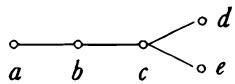
\includegraphics[keepaspectratio]{images/part001_959a1795.jpg}}

represents a graph whose vertices are \(a, b, c, d, e\) and whose edges are \(\{a, b\}\) , \(\{b, c\}\) , \(\{c, d\}\) and \(\{c, e\}\) .

\appendixitem{THE CONNECTED COMPONENTS OF A GRAPH}

Let \(\Gamma = (\mathbf{A},\mathbf{S})\) be a graph. If \(a\) and \(b\) are two vertices, a path joining \(a\) and \(b\) is a sequence \((x_0,\ldots ,x_n)\) of vertices of \(\Gamma\) with \(x_0 = a,x_n = b\) , the vertices \(x_{i}\) and \(x_{i + 1}\) being joined for \(0\leqslant i < n\) ; the integer \(n\geqslant 0\) is the length of the path. The path \((x_0,\ldots ,x_n)\) is said to be injective if \(x_{i}\neq x_{j}\) if \(i\neq j\) . If a path \((x_0,\ldots ,x_n)\) joining \(a\) and \(b\) is of minimal length among such paths, it is necessarily injective; for if not, there would exist i and j with \(0 \leqslant i < j \leqslant n\) and \(x_{i} = x_{j}\) and then the sequence

\[
\left(x _ {0}, \dots , x _ {i}, x _ {j + 1}, \dots , x _ {n}\right)
\]

would be a path of length \textless{} n joining a and b.

The relation ``there exists a path joining a and b'' between two vertices a and b of \(\Gamma\) is an equivalence relation R on the set S of vertices. The equivalence classes of R are called the connected components of \(\Gamma\) ; and \(\Gamma\) is said to be connected if S has at most one connected component, that is if any two vertices of \(\Gamma\) can be joined by at least one path.

PROPOSITION 1. Let \(\Gamma = (A, S)\) be a graph and \((S_{\alpha})_{\alpha \in L}\) its family of connected components. Denote by \(\Gamma_{\alpha}\) the full subgraph of \(\Gamma\) having \(S_{\alpha}\) as its set of vertices.

\begin{enumerate}
\def\labelenumi{(\roman{enumi})}
\item
  For any \(\alpha\) in L, the graph \(\Gamma_{\alpha}\) is connected.
\item
  If \(\Gamma' = (A', S')\) is a connected subgraph of \(\Gamma\) , there exists \(\alpha\) in L such that \(\Gamma' \subset \Gamma_{\alpha}\) .
\item
  If \(\alpha \neq \beta\) , no element of \(S_{\alpha}\) is joined in \(\Gamma\) to any element of \(S_{\beta}\) (equivalently, every edge of \(\Gamma\) is an edge of one of the \(\Gamma_{\alpha}\) ).
\item
  Let \((\mathrm{S}_{\lambda}^{\prime})_{\lambda \in \mathbb{M}}\) be a partition of \(S\) such that, if \(\lambda \neq \mu\) , no element of \(\mathrm{S}_{\lambda}^{\prime}\) is joined in \(\Gamma\) to any element of \(\mathrm{S}_{\mu}^{\prime}\) ; then each of the sets \(\mathrm{S}_{\lambda}^{\prime}\) is a union of connected components of \(\Gamma\) .
\item
  Let \(\alpha\) be in L and \(a\) and \(b\) be in \(S_{\alpha}\) . Then there exists a path \(c = (x_0, \ldots, x_n)\) joining \(a\) and \(b\) in \(\Gamma\) . For any \(i\) with \(0 \leqslant i \leqslant n\) , the path \((x_0, \ldots, x_i)\) joins \(a\) to \(x_i\) in \(\Gamma\) , so \(x_i \in S_{\alpha}\) . Thus, \(c\) is a path in \(\Gamma_{\alpha}\) joining \(a\) and \(b\) . It follows that \(\Gamma_{\alpha}\) is connected.
\item
  Let \(\Gamma' = (A', S')\) be a non-empty connected subgraph of \(\Gamma\) , let \(a\) be an element of \(S'\) and let \(S_{\alpha}\) be the connected component of \(S\) containing \(a\) . For any \(b\) in \(S'\) , there exists a path \(c\) joining \(a\) and \(b\) in \(\Gamma'\) , and \(a\) fortiori in \(\Gamma\) . It follows that \(S' \subset S_{\alpha}\) .
\item
  Given distinct elements \(\alpha\) and \(\beta\) of \(L\) , and vertices \(a \in S_{\alpha}\) and \(b \in S_{\beta}\) , there is no path joining \(a\) and \(b\) , and in particular no edge joining \(a\) and \(b\) .
\item
  Let \(a\) be in \(S_{\lambda}'\) and let \(S_{\alpha}\) be the connected component of \(\Gamma\) containing \(a\) . Then, for any \(b\) in \(S_{\alpha}\) , there exists a path \((x_0, \ldots, x_n)\) joining \(a\) and \(b\) in \(\Gamma\) . If \(i\) is an integer such that \(0 \leqslant i < n\) and if \(x_i \in S_{\lambda}'\) , then \(x_{i+1} \in S_{\lambda}'\) since \(x_i\) is joined to \(x_{i+1}\) . It follows by induction that \(x_i \in S_{\lambda}'\) for \(0 \leqslant i \leqslant n\) , and in particular that \(b = x_n\) is in \(S_{\lambda}'\) . Thus, \(S_{\alpha} \subset S_{\lambda}'\) .
\end{enumerate}

COROLLARY 1. A graph \(\Gamma = (A, S)\) is connected if and only if there does not exist a partition \((S', S'')\) of \(S\) into two non-empty subsets such that no element of \(S'\) is joined in \(\Gamma\) to any element of \(S''\) .

Suppose that \(\Gamma\) is not connected and let \(S'\) be one of its connected components. The set \(S'' = S - S'\) is non-empty by Prop. 1, (i) and no element of \(S'\) is joined to any element of \(S''\) by Prop. 1, (iii).

Suppose now that \(\Gamma\) is connected and let \((S', S'')\) be a partition with the stated property. By Prop. 1, (iv), the set \(S'\) contains at least one connected component, so \(S' = S\) and \(S'' = \varnothing\) , a contradiction.

COROLLARY 2. A subset \(S'\) of \(S\) is a union of connected components if and only if no vertex belonging to \(S'\) is joined to any vertex belonging to \(S - S'\) .

The condition is sufficient by Prop. 1, (iv). It is necessary by Prop. 1, (iii).

